\documentclass[11pt]{article}

\usepackage[a4paper,margin=0.85in]{geometry}
\usepackage[T1]{fontenc}
\usepackage[utf8]{inputenc}
\usepackage{lmodern}
\usepackage{microtype}
\usepackage{amsmath,amssymb,mathtools}
\usepackage{booktabs,longtable,array,tabularx}
\usepackage{enumitem}
\usepackage{xcolor}
\usepackage{hyperref}
\usepackage{graphicx}
\usepackage{caption}
\captionsetup{hypcap=false}
\usepackage{listings}
\usepackage{titlesec}
\usepackage{fancyhdr}
\AtBeginEnvironment{longtable}{\setlength{\parskip}{0pt}}
\setlength{\headheight}{14pt}

\definecolor{ink}{HTML}{111111}
\definecolor{muted}{HTML}{4A5568}
\definecolor{rulegray}{HTML}{D9DEE7}
\definecolor{teal}{HTML}{1F7A74}
\definecolor{bluegray}{HTML}{334E68}
\definecolor{amber}{HTML}{A86D14}
\definecolor{codebg}{HTML}{F7F8FA}

\hypersetup{
  colorlinks=true,
  linkcolor=bluegray,
  citecolor=bluegray,
  urlcolor=bluegray,
  pdftitle={Final Architectural Note: RBCCPS Measurement Block},
  pdfauthor={RBCCPS Streetlight Auditing Project}
}

\lstdefinestyle{clean}{
  backgroundcolor=\color{codebg},
  basicstyle=\ttfamily\footnotesize,
  breaklines=true,
  frame=single,
  rulecolor=\color{rulegray},
  showstringspaces=false,
  tabsize=2,
  columns=fullflexible
}
\lstset{style=clean}

\titleformat{\section}{\Large\bfseries\color{ink}}{\thesection.}{0.6em}{}
\titleformat{\subsection}{\large\bfseries\color{ink}}{\thesubsection}{0.6em}{}
\titleformat{\subsubsection}{\normalsize\bfseries\color{ink}}{\thesubsubsection}{0.6em}{}
\titlespacing*{\section}{0pt}{1.2em}{0.5em}
\titlespacing*{\subsection}{0pt}{0.9em}{0.3em}
\titlespacing*{\subsubsection}{0pt}{0.7em}{0.25em}

\pagestyle{fancy}
\fancyhf{}
\lhead{RBCCPS Measurement Block}
\rhead{Final Architecture Note}
\cfoot{\thepage}
\renewcommand{\headrulewidth}{0.4pt}

\setlength{\parindent}{0pt}
\setlength{\parskip}{0.55em}
\setlist[itemize]{leftmargin=1.2em,itemsep=0.2em,topsep=0.3em}
\setlist[enumerate]{leftmargin=1.4em,itemsep=0.2em,topsep=0.3em}
\renewcommand{\arraystretch}{1.18}
\raggedbottom

\newcommand{\R}{\mathcal{R}}
\newcommand{\I}{\mathcal{I}}
\newcommand{\D}{\mathcal{D}}
\newcommand{\C}{\mathcal{C}}
\newcommand{\G}{\mathcal{G}}
\newcommand{\M}{\mathcal{M}}
\newcommand{\Q}{\mathcal{Q}}
\newcommand{\A}{\mathcal{A}}
\newcommand{\U}{\mathcal{U}}
\newcommand{\OmegaSet}{\Omega}
\newcommand{\given}{\,|\,}

\begin{document}

\pagenumbering{gobble}
\begin{titlepage}
\centering
\vspace*{1.4cm}
{\LARGE\bfseries Final Architectural Note\\[0.25em]}
{\Large\bfseries Measurement Block for the RBCCPS Streetlight Auditing System\\[0.9em]}
{\large Uncertainty-Aware Per-Lamp Useful-Illumination Attribution\\[1.4em]}
\vfill
\begin{minipage}{0.84\textwidth}
\small
\textbf{Scope.} This document consolidates the full system design generated in the design discussion, the internal machine-learning architecture modulations proposed for novelty, and the system-level adoptions selected after reviewing the deep research report. The upstream object-detection block is treated only as an external detection and tracking provider. The contribution specified here is the measurement block.
\end{minipage}
\vfill
{\small Generated as a standalone LaTeX architecture note.}
\end{titlepage}

\pagenumbering{roman}
\tableofcontents
\newpage
\pagenumbering{arabic}

\section{Executive summary}

The RBCCPS measurement block is a structured, stateful, uncertainty-aware system for estimating per-lamp useful illumination from nighttime video, camera metadata, GPS/IMU signals, optional calibration, and tracked streetlight detections. It does not redesign the detector. The detector is an upstream module that produces streetlight boxes, scores, and track identifiers. The measurement block consumes these hypotheses and estimates whether each tracked lamp plausibly provides useful illumination to relevant public-space regions.

The system deliberately does not claim exact lux or luminance from arbitrary compressed phone video. Ordinary phone video is affected by auto-exposure, ISO gain, white balance, HDR, night mode, tone mapping, compression, saturation, motion blur, optical flare, lens bloom, and device-specific ISP behavior. Therefore, uncalibrated video supports proxy useful-illumination assessment, not formal photometry. Optional physical estimates are emitted only under sufficient calibration and field-reference conditions.

The target output is a per-lamp report containing lamp status, plausible affected region, region-wise coverage proxy, adequacy proxy, uniformity proxy, glare penalty, confounder penalty, occlusion penalty, temporal stability, attribution confidence, calibrated confidence, uncertainty flags, and optional physical estimates when permitted. The central research problem is not simply detecting streetlights or measuring brightness. The central problem is attributing useful public-space illumination to a specific lamp under weak geometry, uncontrolled capture, and mixed nighttime light sources.

This architecture combines two layers. The first layer is the disciplined system layer adopted from the deep research report: clip-centered input/output contracts, calibration-tier claim policy, original-frame measurement path, observation-completeness flags, track-pass-inventory state hierarchy, asymmetric scheduling, layered dataset design, leakage-safe evaluation, and traceable reporting. The second layer is the novelty layer developed in this chat: metadata-conditioned radiometric inversion, latent lamp emission-state inference, illumination-disentangled segmentation, lamp-conditioned footprint fields, neural source/confounder decomposition, task-supervised illumination decomposition, distributional coverage and uniformity estimation, counterfactual lamp attribution, monotonic scene-graph fusion, group-conditioned conformal calibration, sparse-reference photometric fields, and route-level graph aggregation.

The strongest research thesis is:
\begin{quote}
Streetlight auditing from nighttime video should be formulated as uncertainty-aware, per-lamp useful-illumination attribution. The key latent variables are lamp emission state, lamp-to-public-space contribution field, non-lamp confounder contribution field, and calibrated uncertainty. A detector-plus-brightness-threshold pipeline is insufficient because it cannot distinguish useful illumination from saturation, glare, headlights, shopfronts, reflections, adjacent lamps, or exposure artifacts.
\end{quote}

The architecture should therefore remain modular and inspectable. It should produce component scores before a final scalar category. It should abstain when uncertainty is high. It should separate proxy mode from calibrated physical mode. It should use learned models internally, but with explicit constraints, monotonicity, counterfactual attribution, and calibration.

\section{Input/output contract}

\subsection{Design principles}

The input/output contract is clip-centered, not merely frame-centered. A reliable measurement requires synchronized video, detector tracks, camera metadata, pose, optional calibration, and state over time. The measurement block must know the original frame coordinate system, capture mode, exposure state, calibration tier, and detector track quality. It must not infer an outage from a missing detection. Missing detection means the lamp was not measured by the upstream detector, not that the lamp was off.

The detector is external. The measurement block requires only a stable detector/tracker contract:
\begin{itemize}
  \item frame identifier and timestamp;
  \item original-frame bounding boxes or explicitly normalized boxes;
  \item streetlight class label;
  \item detector confidence;
  \item stable track identifier;
  \item track confidence, age, and lost-count where available;
  \item optional detector cue scores such as trajectory, size progression, light-characteristics, and position-prior scores.
\end{itemize}

The measurement block performs all measurement on the original capture path. Enhancement and Retinex-style views may be used only as auxiliary inputs for segmentation, confounder handling, or scene parsing. They must not be used as the primary brightness or physical-estimation source.

\subsection{Calibration and claim tiers}

The system uses a calibration-tier policy. The policy is operationally simple but can be implemented with a finer internal scale.

\begin{center}
\small
\begin{tabular}{p{0.13\textwidth}p{0.25\textwidth}p{0.30\textwidth}p{0.21\textwidth}}
\toprule
\textbf{Tier} & \textbf{Capture condition} & \textbf{Allowed claims} & \textbf{Disallowed claims} \\
\midrule
Tier 0 & Ordinary compressed SDR video, uncontrolled auto-exposure, auto white balance, HDR/night-mode unknown. & Lamp status, affected-region proxy, coverage proxy, adequacy category, uniformity proxy, glare/confounder penalties, confidence, uncertainty flags. & Absolute lux or luminance; standards compliance; certification-style pass/fail. \\
Tier 1 & Camera2 or equivalent YUV with per-frame metadata, stable mount, partial capture control. & Stronger relative brightness features, better ranking, robust proxy reports, optional physical-lite indices with very wide uncertainty. & Exact lux; certification claims. \\
Tier 2 & RAW or tightly controlled YUV, known intrinsics, mount calibration, response calibration, vignetting profile, field reference meters. & Optional approximate horizontal/vertical illuminance fields and served-area estimates with uncertainty. & Replacement for formal lighting-engineering survey. \\
Tier 3+ & Controlled research photometry with repeated field references, geometry, and device calibration. & Standards-aware screening with explicit uncertainty and audit caveats. & Automatic legal compliance certification without professional validation. \\
\bottomrule
\end{tabular}
\end{center}

Internally, the implementation may preserve a 0-to-4 calibration scale:
\begin{itemize}
  \item Level 0: no calibration;
  \item Level 1: metadata-only exposure awareness;
  \item Level 2: device profile with intrinsics, response model, and vignetting;
  \item Level 3: device profile plus field lux references under the same capture mode;
  \item Level 4: controlled photometric setup with RAW/linear capture and validated reference measurements.
\end{itemize}

The report layer maps these internal levels into the external claim policy. This combines the fine-grained calibration control from the current design with the stricter allowed/disallowed claim table adopted from the deep research report.

\subsection{Input schema}

A practical clip-centered input schema is:

\begin{lstlisting}
{
  "clip_id": "drive_2026_05_18_001",
  "device_id": "phone_main_wide",
  "calibration_level": 1,
  "policy_id": "rbccps_measurement_policy_v1",
  "frames": [
    {
      "frame_id": 1024,
      "timestamp_ns": 1782837331200000000,
      "image_uri": "frames/frame_001024.yuv",
      "image_format": "YUV_420_888",
      "width": 1920,
      "height": 1080,
      "camera": {
        "exposure_time_s": 0.0167,
        "sensor_sensitivity_iso": 800,
        "aperture_f_number": 1.8,
        "focal_length_mm": 5.4,
        "white_balance_mode": "auto",
        "white_balance_gains": [2.1, 1.0, 1.0, 1.6],
        "ae_mode": "auto",
        "awb_mode": "auto",
        "hdr_mode": "unknown",
        "night_mode": false,
        "digital_zoom": 1.0,
        "ois_eis_enabled": true,
        "metadata_quality": "partial"
      },
      "pose": {
        "latitude": 12.9716,
        "longitude": 77.5946,
        "altitude_m": 900.0,
        "gps_accuracy_m": 4.5,
        "speed_mps": 5.4,
        "heading_deg": 82.0,
        "orientation_quat": [0.1, 0.2, 0.3, 0.9],
        "imu_quality": "good"
      }
    }
  ],
  "tracks": [
    {
      "frame_id": 1024,
      "timestamp_ns": 1782837331200000000,
      "track_id": "track_17",
      "class_name": "streetlight",
      "bbox_xyxy": [814.2, 122.5, 849.7, 171.3],
      "bbox_format": "pixel_xyxy_original_frame",
      "detector_score": 0.79,
      "track_confidence": 0.72,
      "track_age": 21,
      "lost_count": 0,
      "source_model": "yolov26m_v3_hpc",
      "optional_cue_scores": {
        "trajectory": 0.74,
        "size_progression": 0.63,
        "light_characteristics": 0.81,
        "position_prior": 0.65
      }
    }
  ],
  "optional_calibration": {
    "intrinsics": {"fx": 1450.0, "fy": 1452.0, "cx": 960.0, "cy": 540.0},
    "distortion": [0.01, -0.03, 0.0, 0.0, 0.0],
    "mount": {"camera_height_m": null, "pitch_deg": null, "yaw_deg": null},
    "photometric": {
      "response_curve_id": null,
      "vignetting_profile_id": null,
      "field_lux_calibration_id": null
    },
    "map_priors": {
      "lamp_inventory_id": null,
      "road_class": null,
      "lamp_height_m": null,
      "arm_length_m": null
    }
  }
}
\end{lstlisting}

The fields that materially affect the model are image format, frame dimensions, exposure time, ISO, aperture, focal length, AE/AWB/HDR/night-mode status, GPS/IMU quality, bounding-box coordinate convention, detector confidence, track stability, calibration level, and map priors. The coordinate convention is a hard validation gate because a pixel-normalized mismatch invalidates all footprint, mask, and attribution estimates.

\subsection{Output schema}

The output separates evidence, component metrics, judgement, confidence, uncertainty, and optional physical estimates.

\begin{lstlisting}
{
  "measurement_run_id": "run_2026_05_18_001",
  "lamp_observation_id": "obs_track_17_pass_001",
  "lamp_track_id": "track_17",
  "mapped_lamp_id": null,
  "clip_id": "drive_2026_05_18_001",
  "time_window": {
    "start_ns": 1782837330000000000,
    "end_ns": 1782837338000000000,
    "num_frames_used": 28,
    "evidence_frames": [1015, 1016, 1017, 1018]
  },
  "geo_summary": {
    "lat": 12.97161,
    "lon": 77.59465,
    "gps_accuracy_m": 5.2,
    "heading_deg": 82.0
  },
  "status": {
    "label": "on",
    "confidence": 0.87,
    "dim_probability": 0.18,
    "occluded_probability": 0.11,
    "flicker_index": 0.04,
    "saturated_flag": true
  },
  "affected_region": {
    "quality": "moderate",
    "image_mask_uri": "outputs/masks/track_17.npz",
    "ground_polygon_geojson": null,
    "region_mix": {
      "road": 0.62,
      "footpath": 0.28,
      "crossing": 0.00,
      "verge": 0.10
    }
  },
  "metrics": {
    "coverage_proxy": 0.58,
    "adequacy_proxy": 0.62,
    "adequacy_class": "marginal_to_adequate",
    "uniformity_proxy": 0.49,
    "dark_hole_fraction": 0.31,
    "glare_penalty": 0.27,
    "confounder_penalty": 0.34,
    "occlusion_penalty": 0.19,
    "temporal_stability": 0.71,
    "attribution_confidence": 0.56,
    "overall_useful_illumination_score": 0.54,
    "overall_category": "marginal"
  },
  "confidence": {
    "overall": 0.61,
    "calibration_level": 1,
    "observation_completeness": 0.78,
    "attribution_class": "mixed"
  },
  "uncertainty_flags": [
    "auto_exposure_active",
    "mixed_light_sources",
    "partial_ground_plane",
    "moderate_detector_confidence"
  ],
  "optional_physical_estimates": {
    "valid": false,
    "reason": "No field lux calibration and auto exposure active.",
    "horizontal_illuminance_lux_mean": null,
    "horizontal_illuminance_lux_interval": null,
    "vertical_illuminance_lux_mean": null,
    "served_area_m2_est": null
  },
  "traceability": {
    "model_versions": {},
    "feature_snapshot_ref": "features/track_17_pass_001.parquet",
    "policy_id": "rbccps_measurement_policy_v1"
  }
}
\end{lstlisting}

The final report can be exported as JSON for auditability, CSV for operational review, GeoJSON for map display, and overlay video for manual quality assurance. The output must preserve uncertainty rather than hiding it. Valid categories include \texttt{unknown} and \texttt{manual\_review\_recommended}.

Figure~\ref{fig:module-reporting} shows how these output fields are assembled into human-readable reports, machine-readable exports, quality flags, and audit-trail artifacts.

\begin{center}
\centering
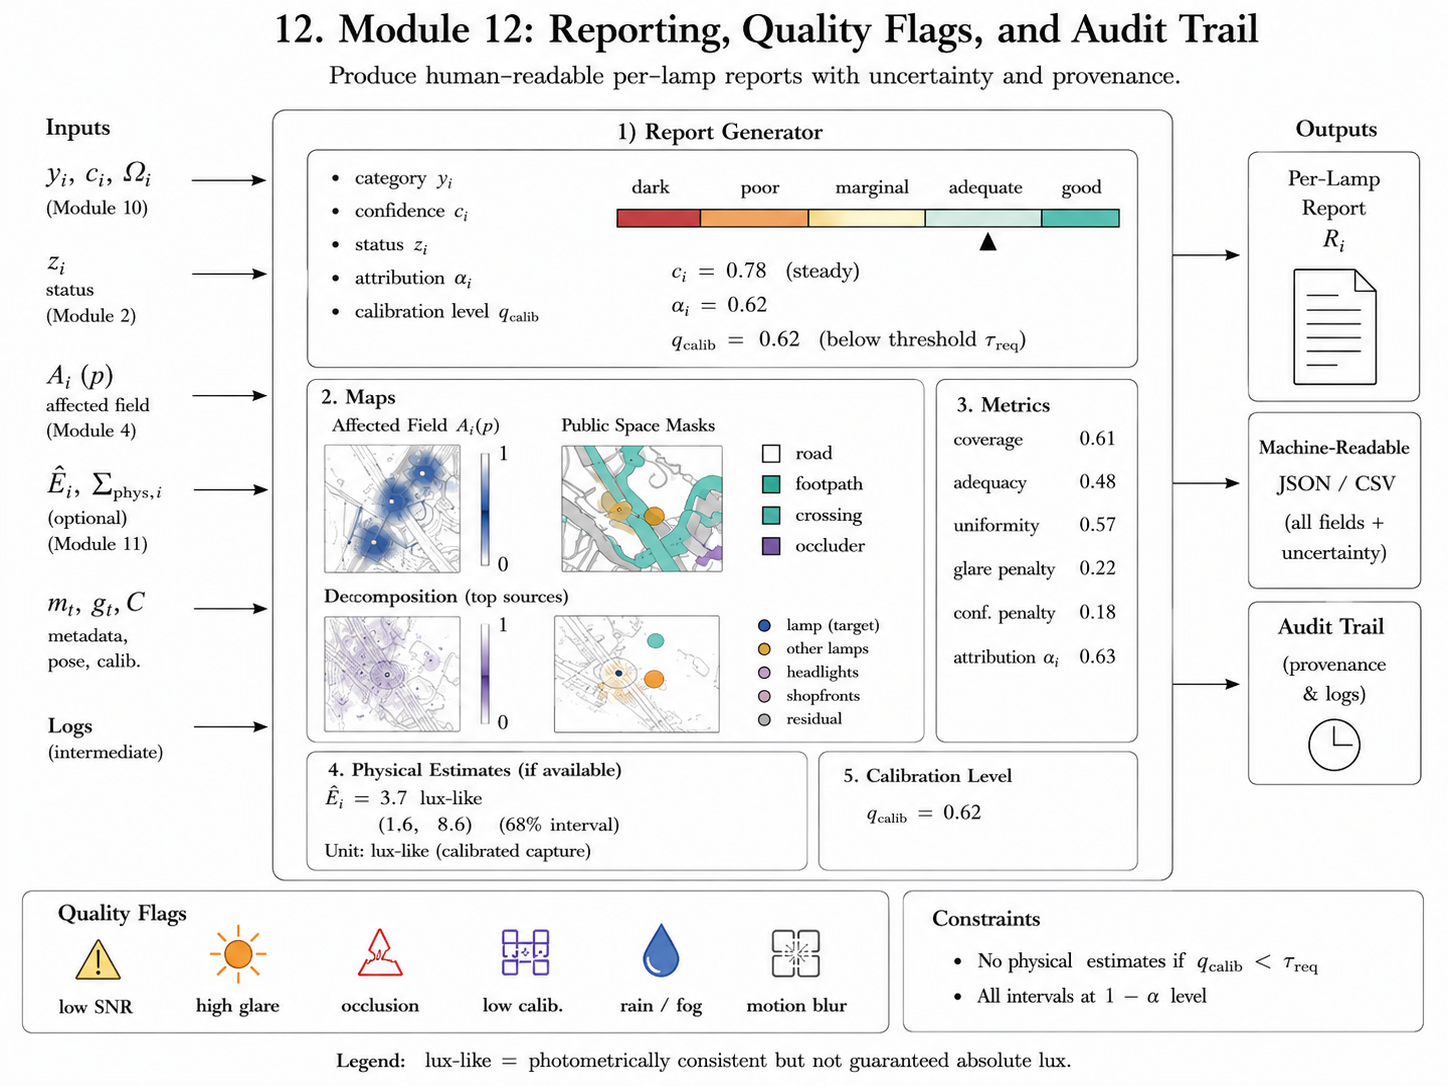
\includegraphics[width=\textwidth]{figures/module_12.png}
\captionof{figure}{Reporting, quality flags, and audit trail. The reporting layer packages status, affected fields, optional physical estimates, calibration level, quality flags, and provenance into per-lamp reports and structured JSON/CSV outputs.}
\label{fig:module-reporting}
\end{center}

This reporting view is the concrete endpoint of the output contract: every downstream municipal or research consumer should receive the same evidence-backed fields rather than an unexplained scalar score.

\section{System architecture: modules, data flow, state, and dependencies}

\subsection{Data flow}

The complete measurement flow is:
\[
(I_t, m_t, g_t, C, D_t)
\rightarrow N_{\theta}
\rightarrow \{S_{\phi}, P_{\psi}, F_{\eta}, D_{\kappa}, T_{\xi}\}
\rightarrow H_{\lambda}
\rightarrow A_{\mathrm{cf}}
\rightarrow G_{\omega}
\rightarrow \Upsilon
\rightarrow \R_i.
\]
Here, \(I_t\) is the frame stream, \(m_t\) is camera metadata, \(g_t\) is GPS/IMU, \(C\) is optional calibration, \(D_t\) is the external detector/tracker output, \(N_{\theta}\) is capture normalization, \(S_{\phi}\) is lamp status inference, \(P_{\psi}\) is public-space segmentation, \(F_{\eta}\) is lamp-conditioned footprint estimation, \(D_{\kappa}\) is source/confounder decomposition, \(T_{\xi}\) is task-supervised reflectance-illumination-source decomposition, \(H_{\lambda}\) is distributional useful-illumination feature estimation, \(A_{\mathrm{cf}}\) is counterfactual attribution, \(G_{\omega}\) is monotonic scene-graph fusion, \(\Upsilon\) is uncertainty/calibration/abstention, and \(\R_i\) is the per-lamp report.

Figure~\ref{fig:measurement-block-overview} provides the end-to-end operator view corresponding to this symbolic flow.

\begin{center}
\centering
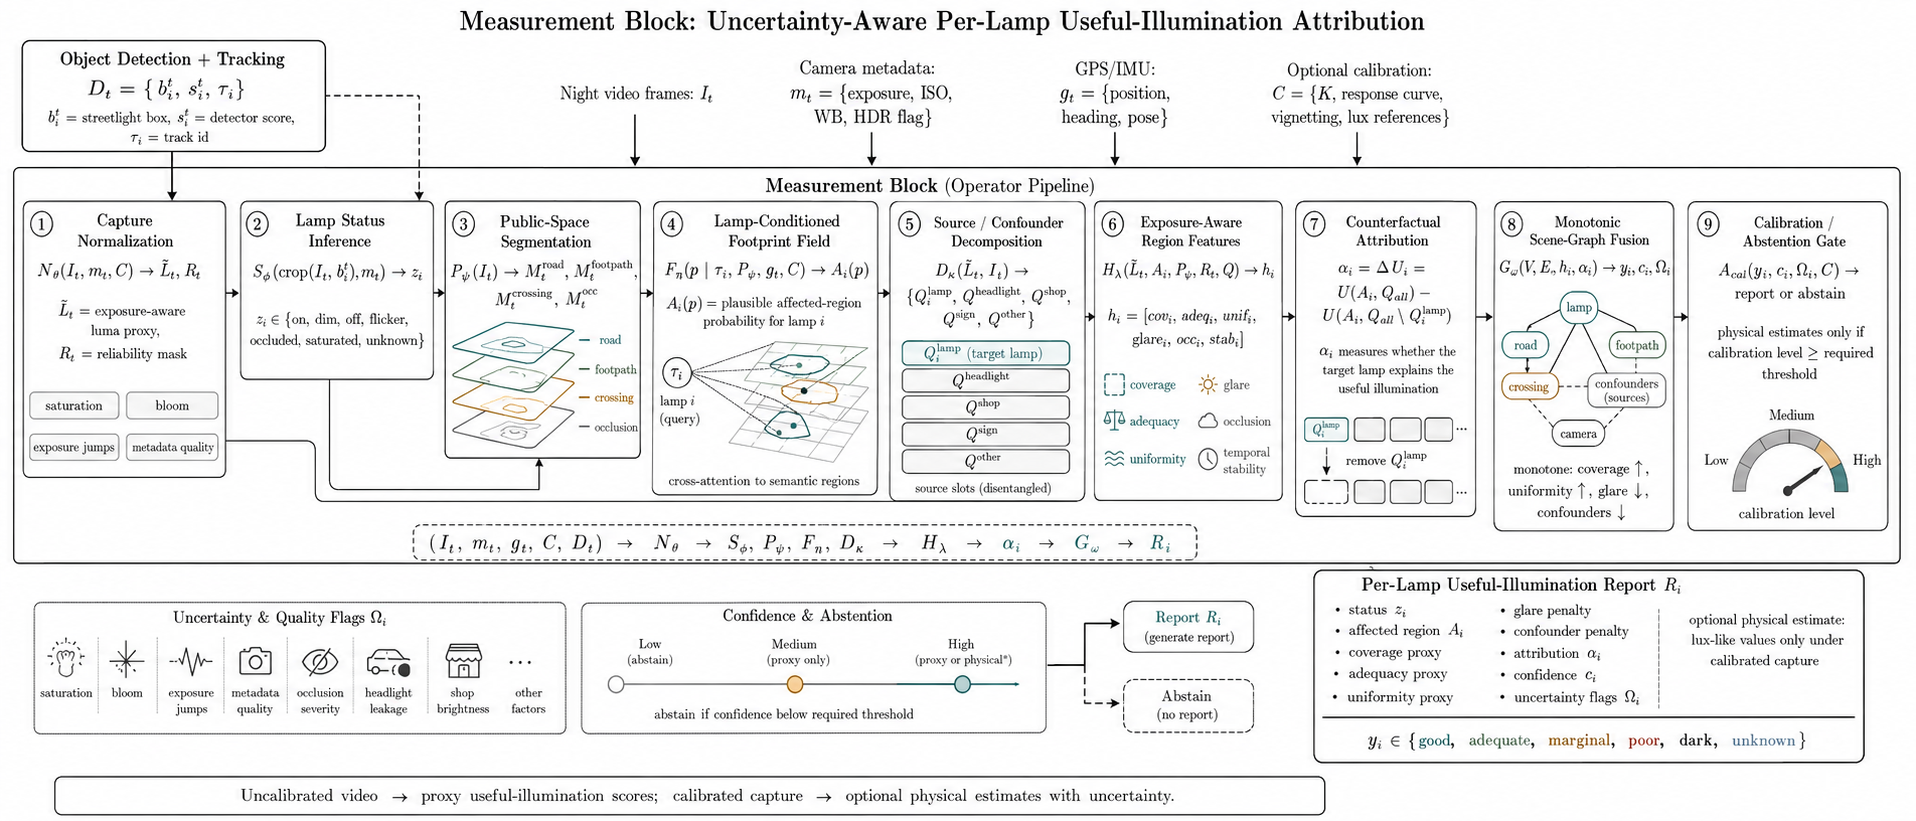
\includegraphics[width=\textwidth]{figures/measurement_block.png}
\captionof{figure}{End-to-end measurement-block architecture. The diagram keeps the upstream detector external, routes original-frame video and metadata through measurement modules, and separates proxy useful-illumination reports from optional calibrated physical estimates.}
\label{fig:measurement-block-overview}
\end{center}

The rest of this section and the algorithmic section unpack the numbered modules in this overview, preserving the same left-to-right dependency structure.

\subsection{Module inventory}

\begin{center}
\scriptsize
\begin{tabular}{p{0.23\textwidth}p{0.31\textwidth}p{0.34\textwidth}}
\toprule
\textbf{Module} & \textbf{Role} & \textbf{Research-level internal architecture} \\
\midrule
Capture normalization & Convert capture stream into an exposure-aware pseudo-linear luma proxy, reliability mask, and uncertainty map. & Metadata-conditioned radiometric inverse with monotonic response curve, device adapters, vignetting correction, saturation intervals, and heteroscedastic uncertainty. \\
Lamp status inference & Estimate on, dim, off, flicker, occluded, saturated, or unknown status over a track window. & Latent emission-state model separating emission, occlusion, capture corruption, and temporal flicker states. \\
Public-space segmentation & Segment road, footpath, crossing, curb, verge, vehicles, vegetation, building, signage, windows, sky, occluders, and unknown regions. & Illumination-disentangled dual-branch segmentation using raw and optional enhanced views, with semantic, nuisance, confounder, and uncertainty decoders. \\
Lamp-conditioned footprint field & Estimate the plausible public-space region served by each target lamp. & Lamp-query to region-token cross-attention field \(A_i(p)\) with geometry, pose, occlusion, and weak distance priors. \\
Source/confounder decomposition & Separate target lamp, other lamps, headlights, shopfronts, signs, signals, reflections, and unknown bright sources. & Slot-attention or mixture-of-experts source decomposition with additive contribution fields \(Q^s(p,t)\). \\
Task-supervised decomposition & Separate reflectance-like structure, illumination-like field, and source-like field. & Three-head decomposition with reconstruction, segmentation-aware, measurement-aware, and source-separation losses. \\
Distributional useful-illumination features & Estimate coverage, adequacy, uniformity, dark holes, glare, occlusion, and stability. & Region-conditioned quantile regression, dark-hole map, adequacy head, uniformity head, and temporal aggregation. \\
Counterfactual attribution & Estimate whether the target lamp explains the useful illumination in its served region. & Counterfactual source suppression: \(\alpha_i = \U(A_i,Q_{all}) - \U(A_i,Q_{all}\setminus Q_i^{lamp})\). \\
Monotonic scene-graph fusion & Fuse component evidence into final class, confidence, and uncertainty set. & Graph neural fusion over lamp, region, confounder, camera, geometry, and route nodes with monotonic output constraints. \\
Conformal uncertainty and abstention & Calibrate prediction sets, confidence, and physical-validity decisions. & Group-conditioned conformal calibration by device, route, capture mode, wetness, and confounder density. \\
Sparse-reference photometric field & Optional calibrated physical field under sufficient calibration. & Neural field over ground-plane coordinates conditioned on source fields, footprint, calibration, and sparse lux references. \\
Route-level aggregation & Merge repeated passes and produce stable map-level reports. & Spatiotemporal graph aggregation over track observations, candidate physical lamps, road segments, and drive passes. \\
\bottomrule
\end{tabular}
\end{center}

\subsection{State hierarchy}

The system is stateful at three levels.

\textbf{Track state.} Each active detector track maintains crop buffers, metadata history, exposure history, normalized brightness features, segmentation references, footprint hypotheses, source/confounder evidence, and uncertainty flags.

\textbf{Pass-level lamp observation state.} Track fragments that likely refer to the same physical lamp within one clip or drive pass are merged into a \texttt{lamp\_observation}. This object stores evidence frames, dominant public-space region, component metrics, confidence, and traceability.

\textbf{Inventory or route-level state.} Repeated observations across passes are optionally merged into candidate physical lamp identities and road-segment underlighting reports. This layer uses GPS neighborhoods, visual similarity, road topology, map priors, and confidence-weighted consensus.

This state hierarchy is an adoption from the deep research report analysis and is retained because it improves both accuracy and deployment stability. Flicker, occlusion, exposure jumps, duplicate tracks, and mixed-source attribution cannot be judged reliably from single frames.

\subsection{Dependencies and scheduling}

The measurement block depends on:
\begin{itemize}
  \item upstream detector/tracker output, treated as a black-box contract;
  \item original video frames, preferably YUV or RAW under controlled capture;
  \item camera metadata, especially exposure, ISO, AE/AWB/HDR/night-mode state, focal length, and frame duration;
  \item GPS/IMU for geo-tagging, heading, pose, and rough ground-plane priors;
  \item optional intrinsics, response curves, vignetting, mount calibration, field lux references, and map priors;
  \item internal learned models for segmentation, radiometric normalization, source decomposition, footprint estimation, attribution, and fusion.
\end{itemize}

The scheduling policy is asymmetric. Detector/tracker outputs are consumed every frame. Lamp status and source/confounder evidence update on short windows. Segmentation and geometry update every few frames or when camera pose changes significantly. Final reports are emitted when a track window closes, when the lamp leaves view, or at a fixed evidence threshold. This improves mobile feasibility without weakening the report-level inference.

\section{Algorithmic design}

\subsection{Capture normalization}

Capture normalization is modeled as:
\[
N_{\theta}(I_t,m_t,C,d) \rightarrow (\widetilde{L}_t,R_t,\Sigma_t),
\]
where \(\widetilde{L}_t\) is the exposure-aware luma proxy, \(R_t\) is a reliability mask, \(\Sigma_t\) is radiometric uncertainty, and \(d\) is a device identifier.

The stronger research formulation uses a constrained camera-response inverse network. The raw frame branch extracts luma and color features. The metadata encoder embeds exposure time, ISO, aperture, white balance, AE/AWB/HDR/night-mode state, focal length, and frame duration. A device embedding and device-conditioned adapter layers handle phone-specific response and ISP differences. A monotonic spline layer approximates the inverse camera response curve. A low-frequency vignetting field corrects spatial brightness falloff when calibration allows it. Saturation and bloom are treated as interval-valued uncertainty, not as valid point measurements.

The constraints are:
\begin{align*}
\frac{d f^{-1}_{\theta}(x)}{dx} &\geq 0, \\
\nabla^2 V_{\theta}(p) &\approx 0 \quad \text{for smooth vignetting}, \\
\widetilde{L}_t(p) &\in [L_{min}(p),L_{max}(p)] \quad \text{for saturated pixels}, \\
\text{physical output} &= \varnothing \quad \text{if calibration is insufficient.}
\end{align*}

The output of this module is not a true radiance estimate in Tier 0 or Tier 1. It is a pseudo-linear, exposure-aware proxy with a reliability map and uncertainty map. All downstream measurement features should either use this proxy or explicitly mark their own weaker validity.

Figure~\ref{fig:module-capture-normalization} expands the capture-normalization path from raw frame and metadata inputs to luma proxy, reliability mask, physical-validity gate, and quality flags.

\begin{center}
\centering
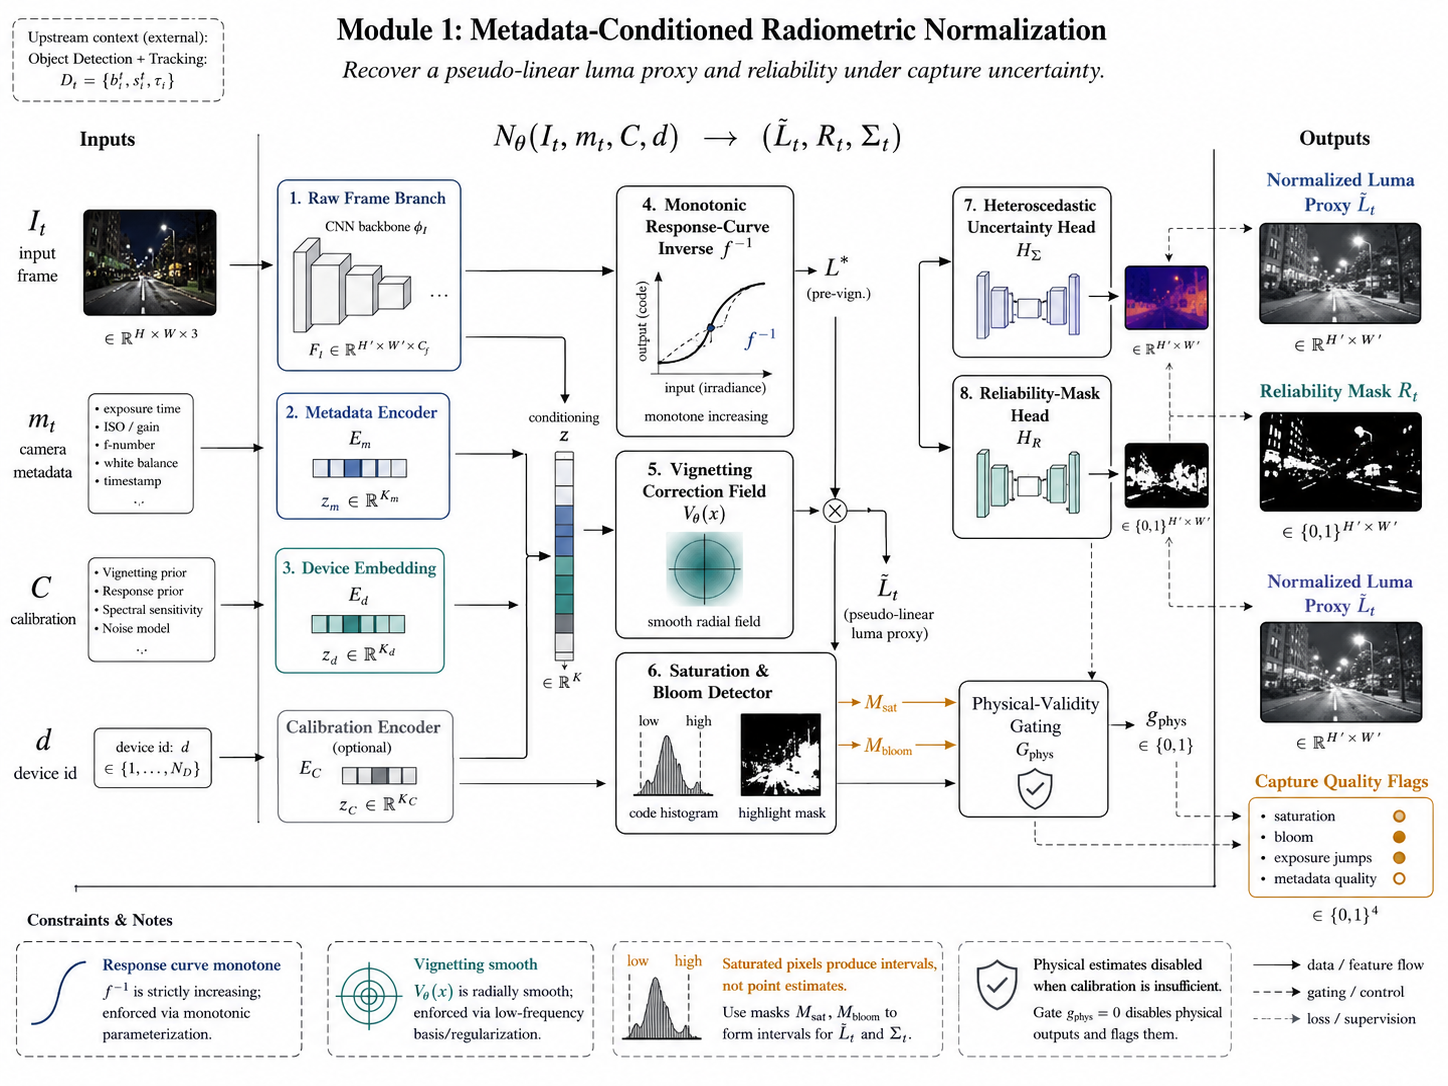
\includegraphics[width=\textwidth]{figures/module_1.png}
\captionof{figure}{Metadata-conditioned radiometric normalization. The module produces an exposure-aware luma proxy and reliability products while explicitly marking saturation, bloom, exposure jumps, and insufficient physical validity.}
\label{fig:module-capture-normalization}
\end{center}

The figure is intended as an implementation pointer for the first preprocessing component: downstream modules should consume the normalized proxy and reliability outputs, not raw brightness alone.

\subsection{Lamp crop and latent emission-state inference}

For each detector track \(\tau_i\), the system extracts a crop sequence around the lamp box \(b_i^t\) and estimates hidden states:
\[
S_{\phi}(\operatorname{crop}(I_t,b_i^t),m_t,R_t)
\rightarrow p(e_i,o_i,q_i,f_i \given \cdot), z_i.
\]
Here \(e_i\) is the intrinsic emission state, \(o_i\) is the occlusion state, \(q_i\) is the capture corruption state, \(f_i\) is the temporal flicker state, and \(z_i\) is the operational status label.

The architecture uses a crop encoder, temporal transformer or state-space model, exposure token, saturation token, occlusion token, and multi-head latent-state outputs. The state decomposition prevents the model from confusing a bright saturated source with a reliable lamp measurement, or an occluded lamp with an off lamp.

The training objective combines:
\[
\mathcal{L}_{status} + \lambda_1\mathcal{L}_{smooth} + \lambda_2\mathcal{L}_{flicker} + \lambda_3\mathcal{L}_{exposure\text{-}inv} + \lambda_4\mathcal{L}_{calib}.
\]
The final status classes are \texttt{on}, \texttt{dim}, \texttt{off}, \texttt{flicker}, \texttt{occluded}, \texttt{saturated}, and \texttt{unknown}. The model should emit posterior probabilities and not only a hard label.

Figure~\ref{fig:module-lamp-status} shows the corresponding crop-sequence architecture and separates emission, occlusion, capture corruption, and flicker states before producing the operational status label.

\begin{center}
\centering
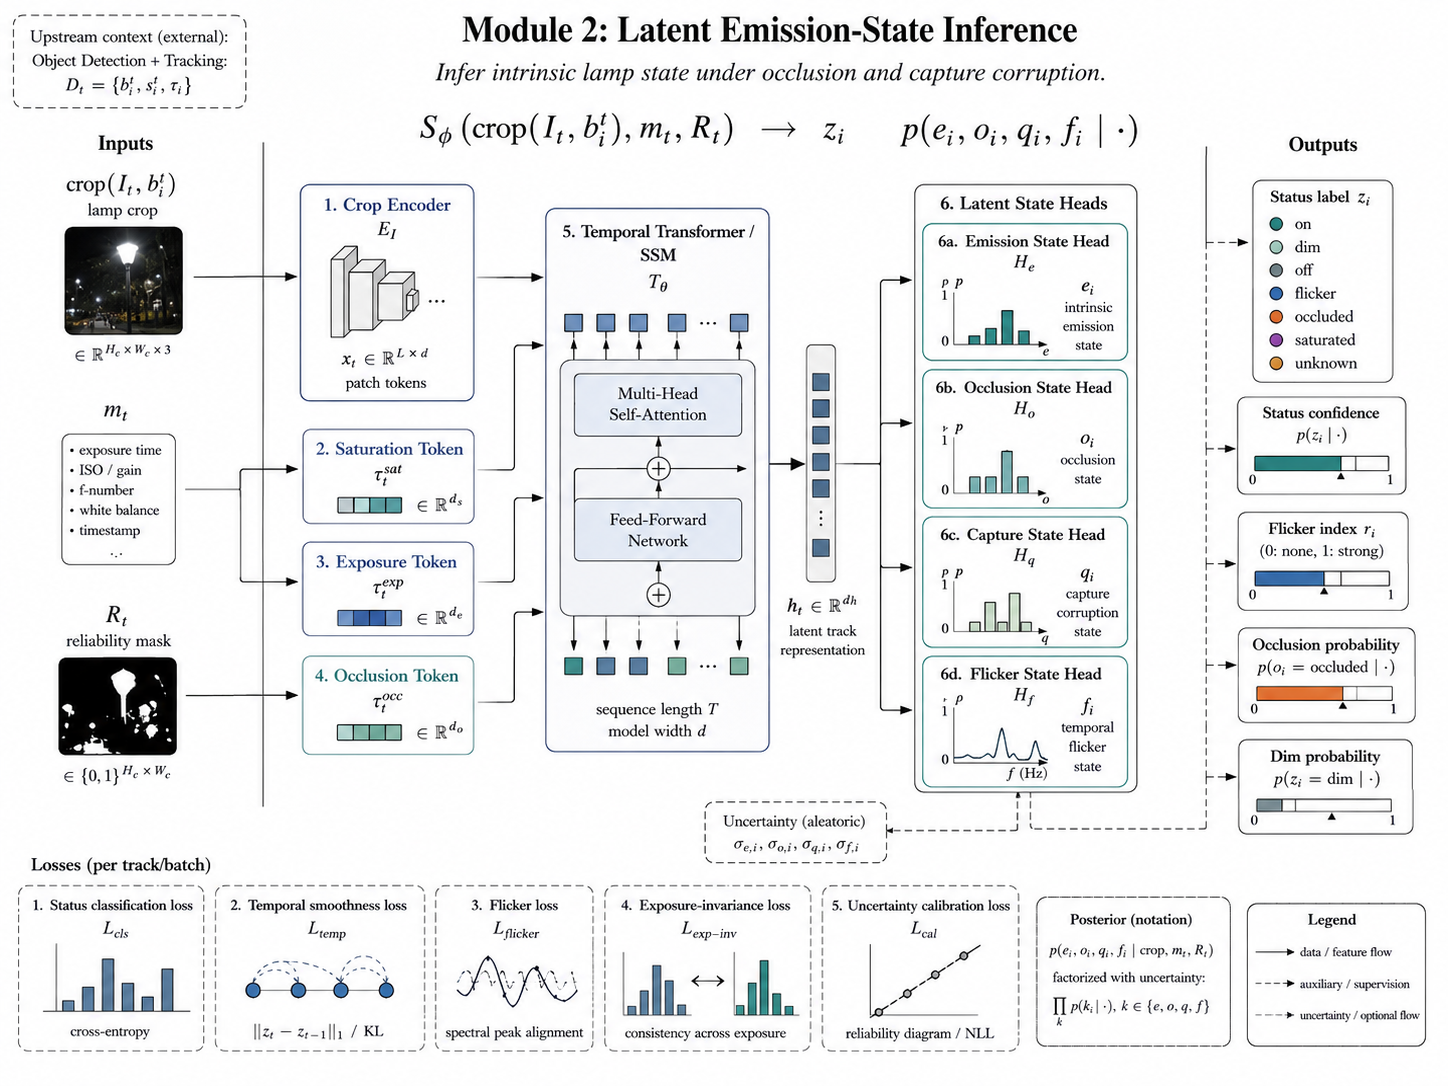
\includegraphics[width=\textwidth]{figures/module_2.png}
\captionof{figure}{Latent emission-state inference. Temporal lamp crops, exposure tokens, saturation tokens, and occlusion tokens feed state heads for emission, occlusion, capture corruption, flicker, confidence, and status.}
\label{fig:module-lamp-status}
\end{center}

This diagram clarifies why the report should preserve probabilities and auxiliary indices such as flicker and occlusion rather than collapsing evidence into a single on/off decision.

\subsection{Illumination-disentangled public-space segmentation}

The segmentation model estimates semantic masks and uncertainty:
\[
P_{\psi}(I_t,I_t^{enh}) \rightarrow \{M_t^k\}_{k=1}^{K}, U_t^{seg}.
\]
The optional enhanced image \(I_t^{enh}\) may be produced by low-light enhancement or Retinex-style processing, but it is used only as an auxiliary view. Measurement features are always sampled from the original or normalized capture path.

The architecture has a raw-image branch, an optional enhanced-view branch, a shared semantic trunk, an illumination-nuisance branch, cross-attention fusion, a public-space decoder, a confounder-aware decoder, and an uncertainty decoder. The goal is to learn semantic structure while reducing dependence on illumination artifacts. A dark footpath should remain a footpath; it should not disappear because it is dark.

Required classes include road, footpath, crossing, curb, verge, vegetation, vehicle, building, shopfront, window, sign, billboard, traffic signal, sky, wet/reflection-like road, occluder, and unknown. Losses include segmentation cross-entropy, boundary loss, exposure perturbation consistency, night-style consistency, uncertainty loss, and confounder separation loss.

Figure~\ref{fig:module-segmentation} places those semantic, public-space, occluder, confounder, and uncertainty outputs into one segmentation module.

\begin{center}
\centering
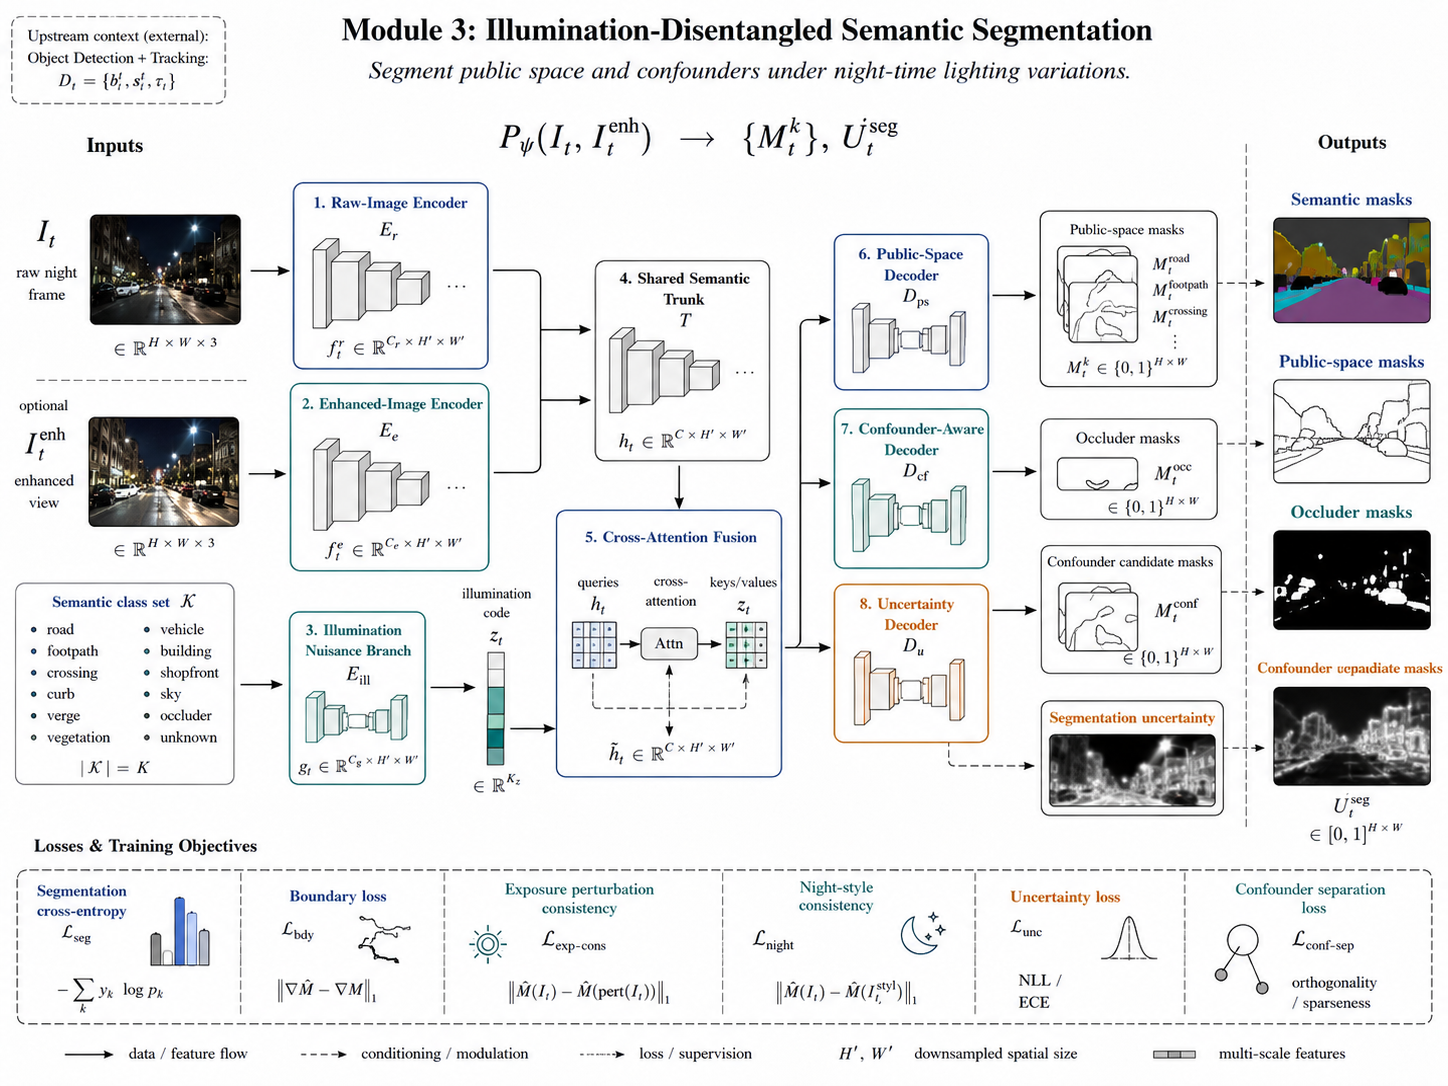
\includegraphics[width=\textwidth]{figures/module_3.png}
\captionof{figure}{Illumination-disentangled semantic segmentation. Raw and optional enhanced views support public-space masks, occluder masks, confounder candidates, and segmentation uncertainty without turning enhancement into measurement evidence.}
\label{fig:module-segmentation}
\end{center}

The key pointer from the figure is that segmentation is a structural support module: it identifies where measurement should be evaluated and where confounders or uncertainty should reduce confidence.

\subsection{Lamp-conditioned affected-region field}

For each target lamp \(i\), the system predicts a soft affected-region field:
\[
F_{\eta}(p\given \tau_i,P_{\psi},g_t,C) \rightarrow A_i(p),
\]
where \(A_i(p)\in[0,1]\) is the probability that public-space point or pixel \(p\) is plausibly served by lamp \(i\).

The architecture treats the lamp as a query token and public-space patches as key/value tokens. It uses lamp track embeddings, bbox sequence features, pose and geometry encodings, semantic patch tokens, optional depth features, occlusion gates, and a weak distance-decay prior. The field is constrained by:
\begin{align*}
A_i(p)&=0 \quad \text{outside public-space masks},\\
A_i(p)&\downarrow \quad \text{under occlusion},\\
\operatorname{Var}(A_i(p))&\uparrow \quad \text{when geometry is weak},\\
A_i(p)&\text{ is softly distance-decaying, not hard-coded.}
\end{align*}

This is a core novelty module. It turns the system from scene-level brightness assessment into per-lamp contribution reasoning.

Figure~\ref{fig:module-affected-region} visualizes this lamp-conditioned affected-region field as cross-attention from a lamp query to public-space patches, with geometry, occlusion, and distance priors acting as soft gates.

\begin{center}
\centering
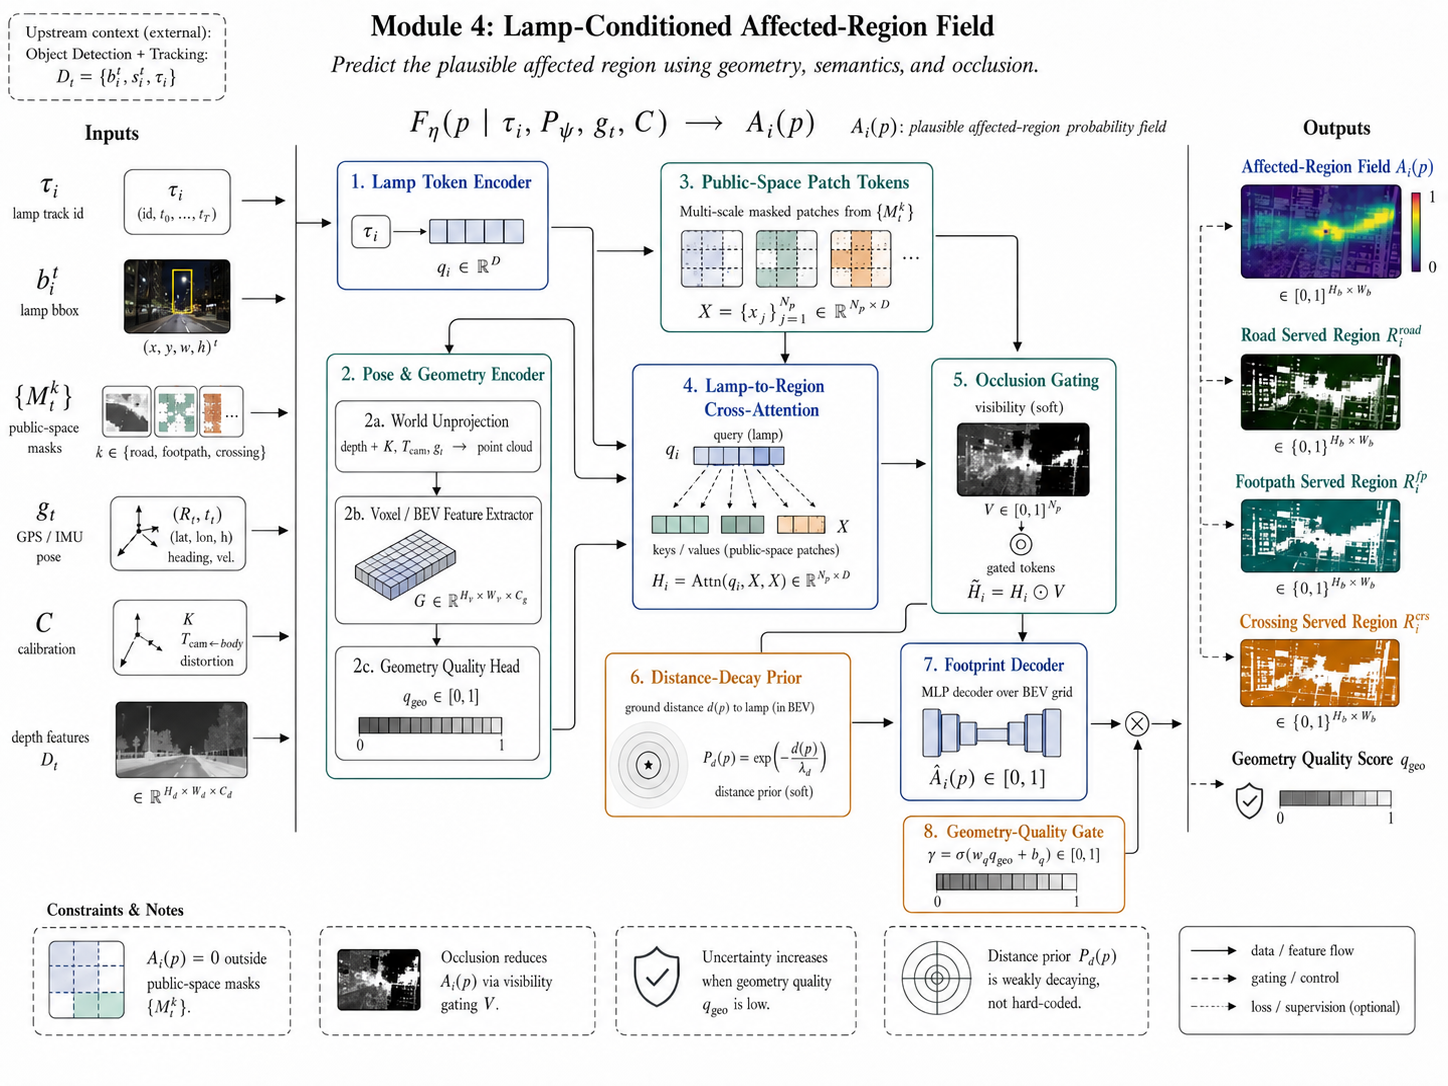
\includegraphics[width=\textwidth]{figures/module_4.png}
\captionof{figure}{Lamp-conditioned affected-region field. The module predicts soft served-region fields for road, footpath, and crossing areas while carrying a geometry-quality score.}
\label{fig:module-affected-region}
\end{center}

This figure should be read as the bridge between detection and measurement: the lamp box is only the query, while the measured target is the public-space region plausibly served by that lamp.

\subsection{Neural source and confounder decomposition}

The source decomposition module estimates source contribution fields:
\[
D_{\kappa}(\widetilde{L}_t,I_t,\text{temporal context})
\rightarrow \{Q_i^{lamp},Q^{otherlamp},Q^{headlight},Q^{shop},Q^{signal},Q^{refl},Q^{unk}\}.
\]
It uses a shared scene encoder, slot-attention or mixture-of-experts block, temporal motion separator, source-type classifier, and source-contribution decoder. The additive interpretation is:
\[
\widetilde{L}_t(p) \approx \sum_{s\in\mathcal{S}} Q^s(p,t) + \epsilon(p,t),
\]
where sources include the target lamp, other lamps, headlights, shopfronts/windows, signals/signage, reflections, and unknown bright sources.

This module is required because attribution fails if bright road or footpath regions are caused by headlights, shops, signs, windows, decorative lights, wet-road reflections, or nearby lamps. Losses include reconstruction, source classification, temporal consistency, slot assignment, sparsity, and disentanglement regularization.

Figure~\ref{fig:module-source-decomposition} shows the source slots and contribution fields used to separate target-lamp evidence from other lamps and non-lamp confounders.

\begin{center}
\centering
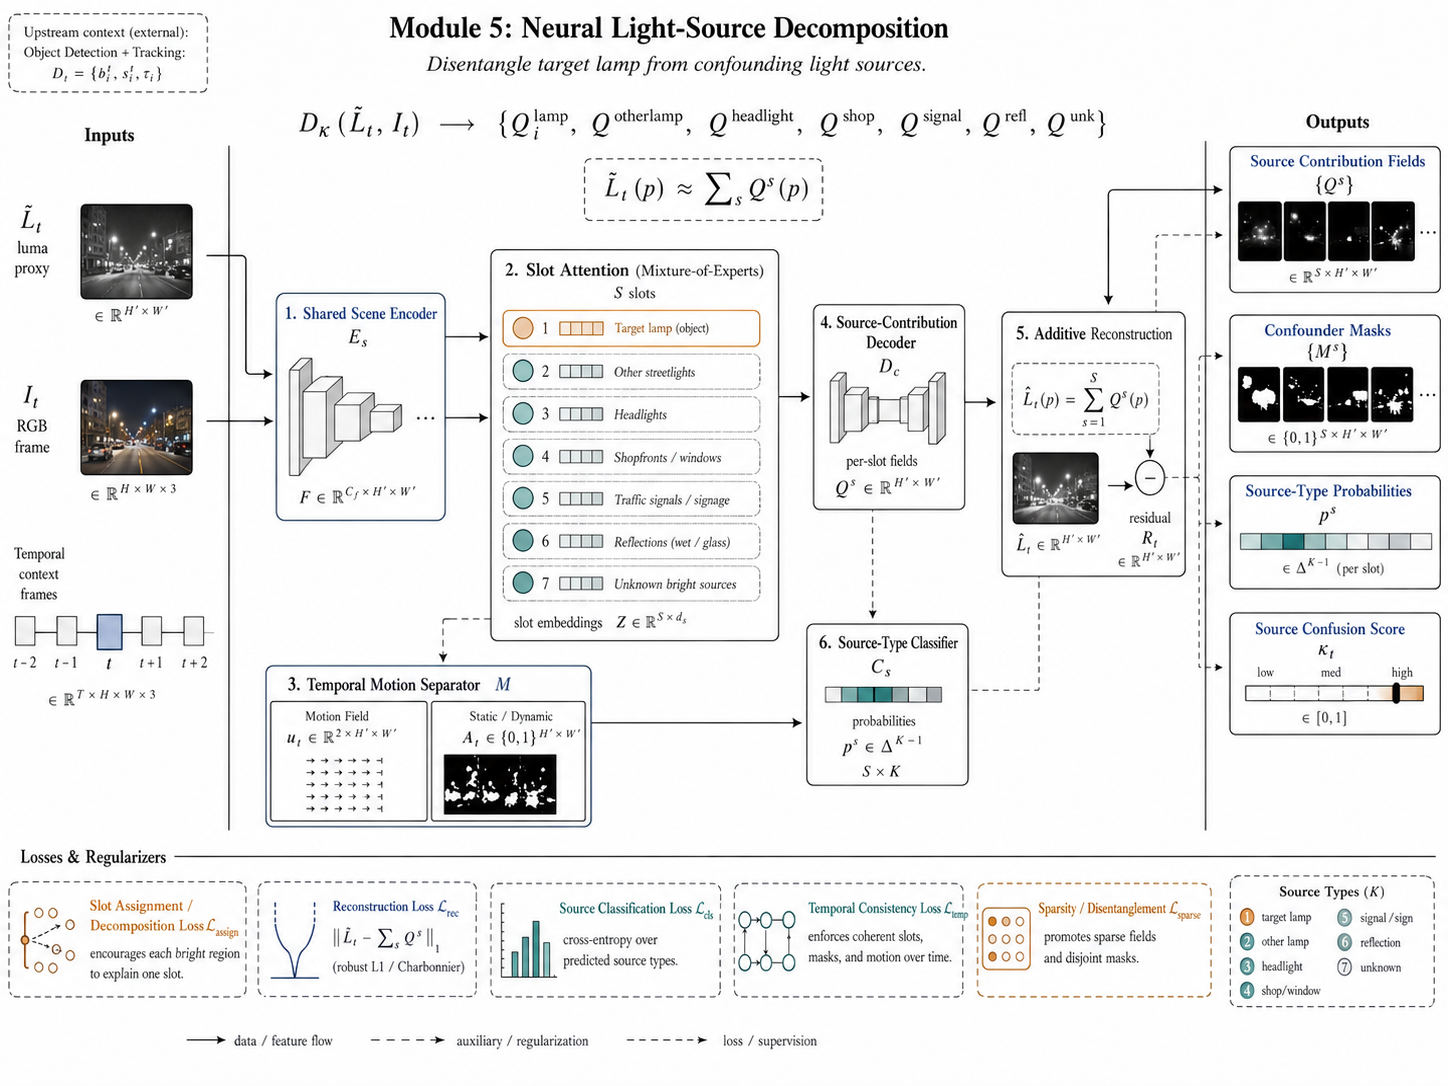
\includegraphics[width=\textwidth]{figures/module_5.png}
\captionof{figure}{Neural light-source decomposition. Slot attention or mixture-of-experts decomposition assigns normalized luma evidence to target lamps, other lamps, headlights, shopfronts, signals, reflections, and unknown sources.}
\label{fig:module-source-decomposition}
\end{center}

The diagram is the operational basis for the confounder penalty and attribution confidence: bright pixels remain useful only if the source decomposition supports the target lamp as the contributor.

\subsection{Task-supervised reflectance-illumination-source decomposition}

The decomposition module predicts:
\[
T_{\xi}(I_t,\widetilde{L}_t) \rightarrow (R_t^{refl},L_t^{illum},S_t^{src}),
\]
with reconstruction:
\[
I_t \approx f(R_t^{refl},L_t^{illum},S_t^{src}).
\]
Here, \(R_t^{refl}\) supports semantic structure, \(L_t^{illum}\) supports coverage and adequacy, and \(S_t^{src}\) supports glare and confounder reasoning. This turns Retinex from a generic preprocessing step into a task-supervised internal representation.

The decomposition is trained with reconstruction loss, decomposition consistency, segmentation-aware loss, measurement-aware loss, and source separation loss. It should not be interpreted as exact physical decomposition in uncalibrated capture.

Figure~\ref{fig:module-ris-decomposition} summarizes this task-supervised decomposition into reflectance-like, illumination-like, and source-like internal fields.

\begin{center}
\centering
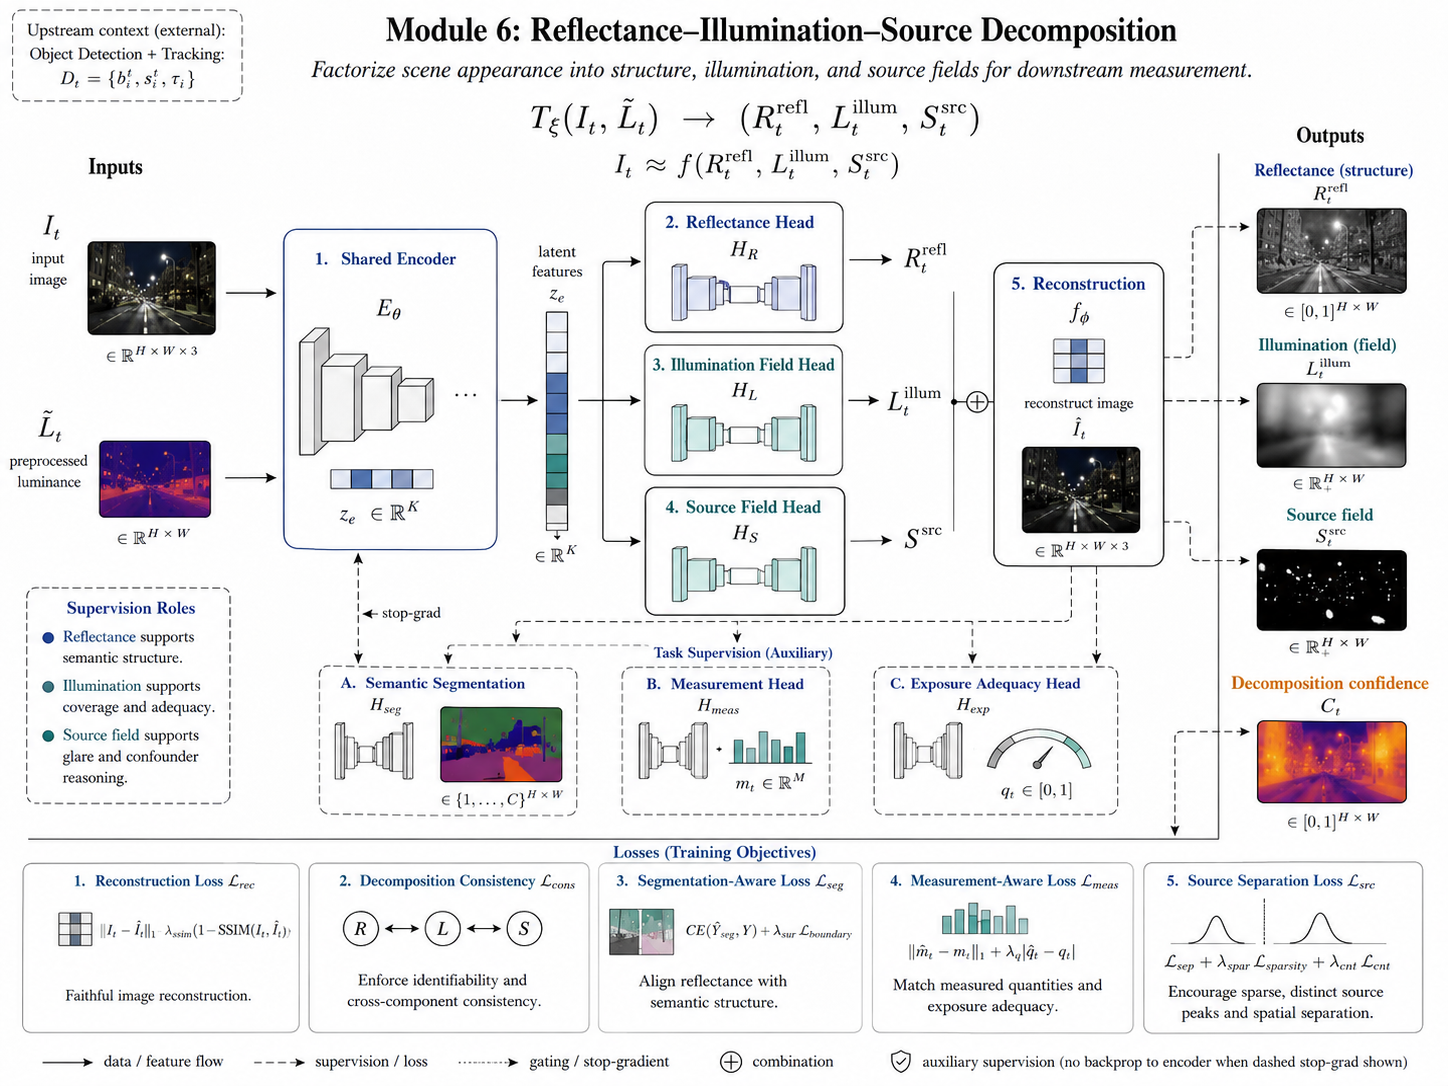
\includegraphics[width=\textwidth]{figures/module_6.png}
\captionof{figure}{Reflectance--illumination--source decomposition. The module factors scene appearance into structure, illumination field, and source field while using reconstruction, segmentation, measurement, exposure, and source-separation supervision.}
\label{fig:module-ris-decomposition}
\end{center}

This visual should be interpreted conservatively: the decomposition is a learned representation for downstream measurement and debugging, not a guarantee of physical Retinex correctness under uncontrolled capture.

\subsection{Distributional useful-illumination features}

The feature estimator predicts a distribution, not only one average brightness value:
\[
H_{\lambda}(\widetilde{L}_t,A_i,P_{\psi},R_t,Q) \rightarrow h_i,
\]
with
\[
 h_i = [cov_i, adeq_i, unif_i, glare_i, occ_i, stab_i].
\]
The model outputs quantiles \(q_{10},q_{25},q_{50},q_{75},q_{90}\), dark-hole probability maps, coverage probability, uniformity score, task-conditioned adequacy, glare, occlusion, and temporal stability.

Coverage is the fraction of accessible target-region pixels whose distributional brightness exceeds a learned or calibrated useful-light threshold. Adequacy is task-conditioned: carriageway, footpath, crossing, and verge require separate interpretation. Uniformity is based on low-percentile behavior and dark-hole structure, not only mean brightness. Glare uses saturation, bloom radius, source angular prominence, and veiling-light proxies. Occlusion uses vegetation, vehicle, building, sign, and frame-truncation masks. Temporal stability is the exposure-normalized consistency of component metrics across the track window.

Figure~\ref{fig:module-distributional-features} expands these component metrics into quantile, dark-hole, uniformity, adequacy, and temporal-stability heads.

\begin{center}
\centering
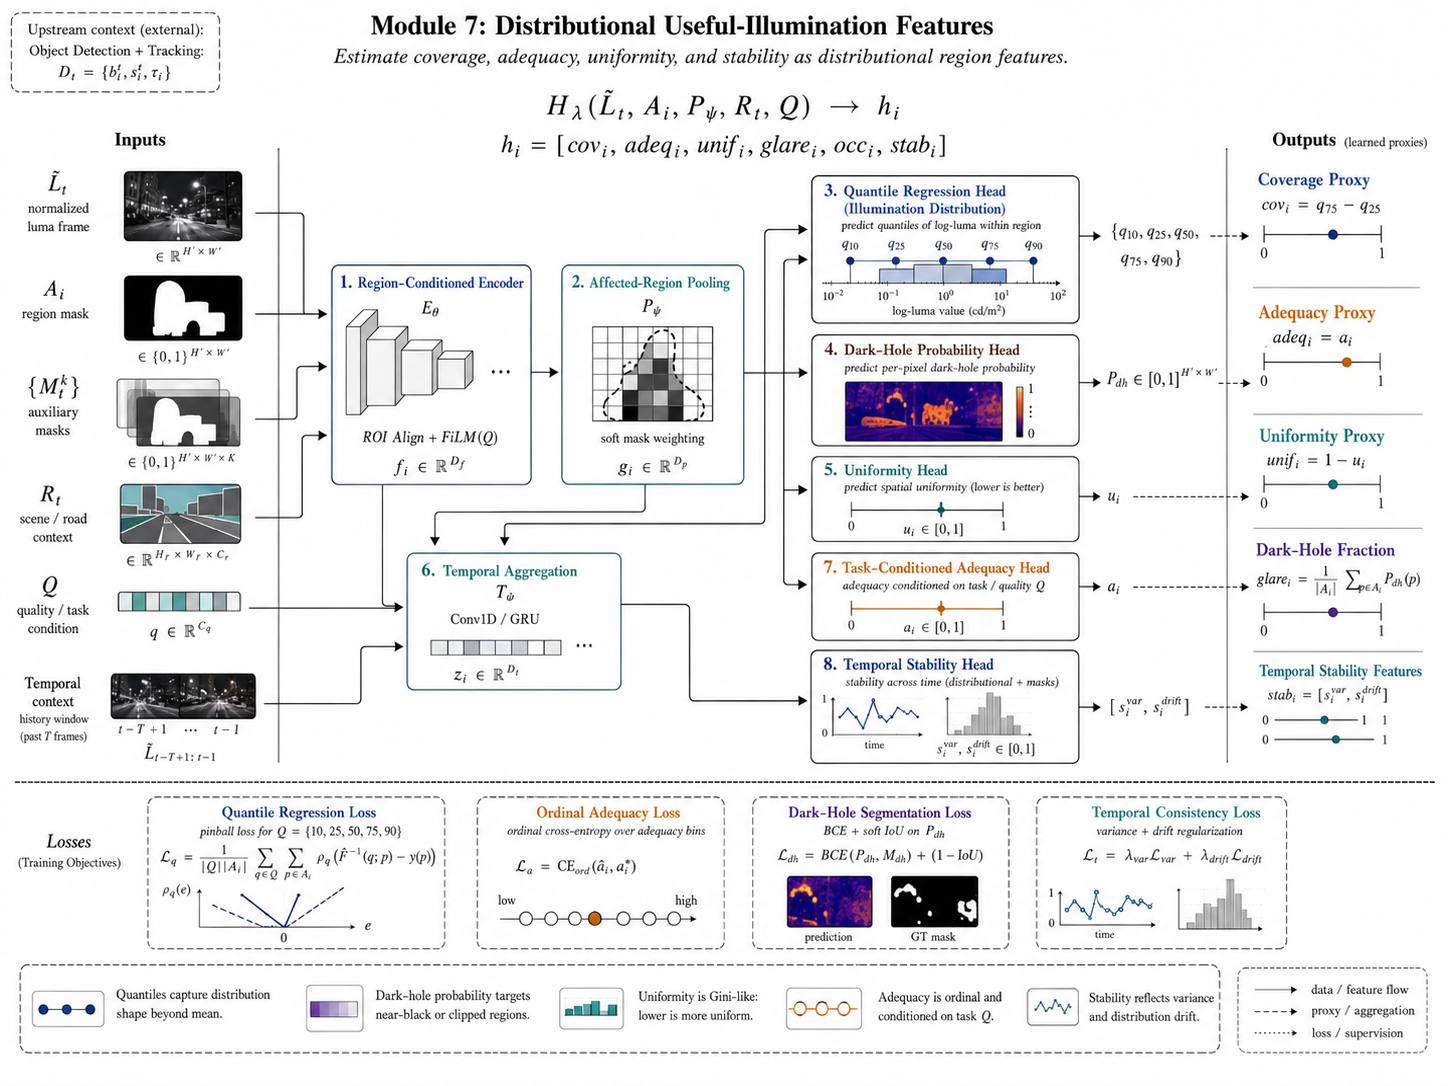
\includegraphics[width=\textwidth]{figures/module_7.png}
\captionof{figure}{Distributional useful-illumination features. The module estimates coverage, adequacy, uniformity, dark-hole behavior, and temporal stability from affected-region features rather than relying on a single mean brightness.}
\label{fig:module-distributional-features}
\end{center}

The implementation pointer is that useful illumination should be represented as a small distributional feature vector before final fusion, which keeps dark holes and unstable evidence visible.

\subsection{Counterfactual lamp attribution}

The attribution model asks whether the target lamp is necessary to explain the useful illumination:
\[
\alpha_i = \Delta U_i = \U(A_i,Q_{all}) - \U(A_i,Q_{all}\setminus Q_i^{lamp}).
\]
Here, \(\U(\cdot)\) is the useful-illumination functional over the affected region, \(Q_{all}\) is the full set of source fields, and \(Q_i^{lamp}\) is the target-lamp source field.

If suppressing the target lamp leaves the served-region utility mostly unchanged, attribution confidence should drop. If the useful illumination collapses when the target lamp contribution is removed, attribution confidence increases. This counterfactual formulation is more rigorous than spatial overlap or brightness correlation alone.

Outputs are attribution score \(\alpha_i\), attribution class \(\{certain,mixed,uncertain\}\), source competition evidence, and counterfactual uncertainty. Losses include attribution classification, counterfactual consistency, and mixed-source ranking losses.

Figure~\ref{fig:module-counterfactual-attribution} shows the all-source and without-target utility comparison that produces the attribution score.

\begin{center}
\centering
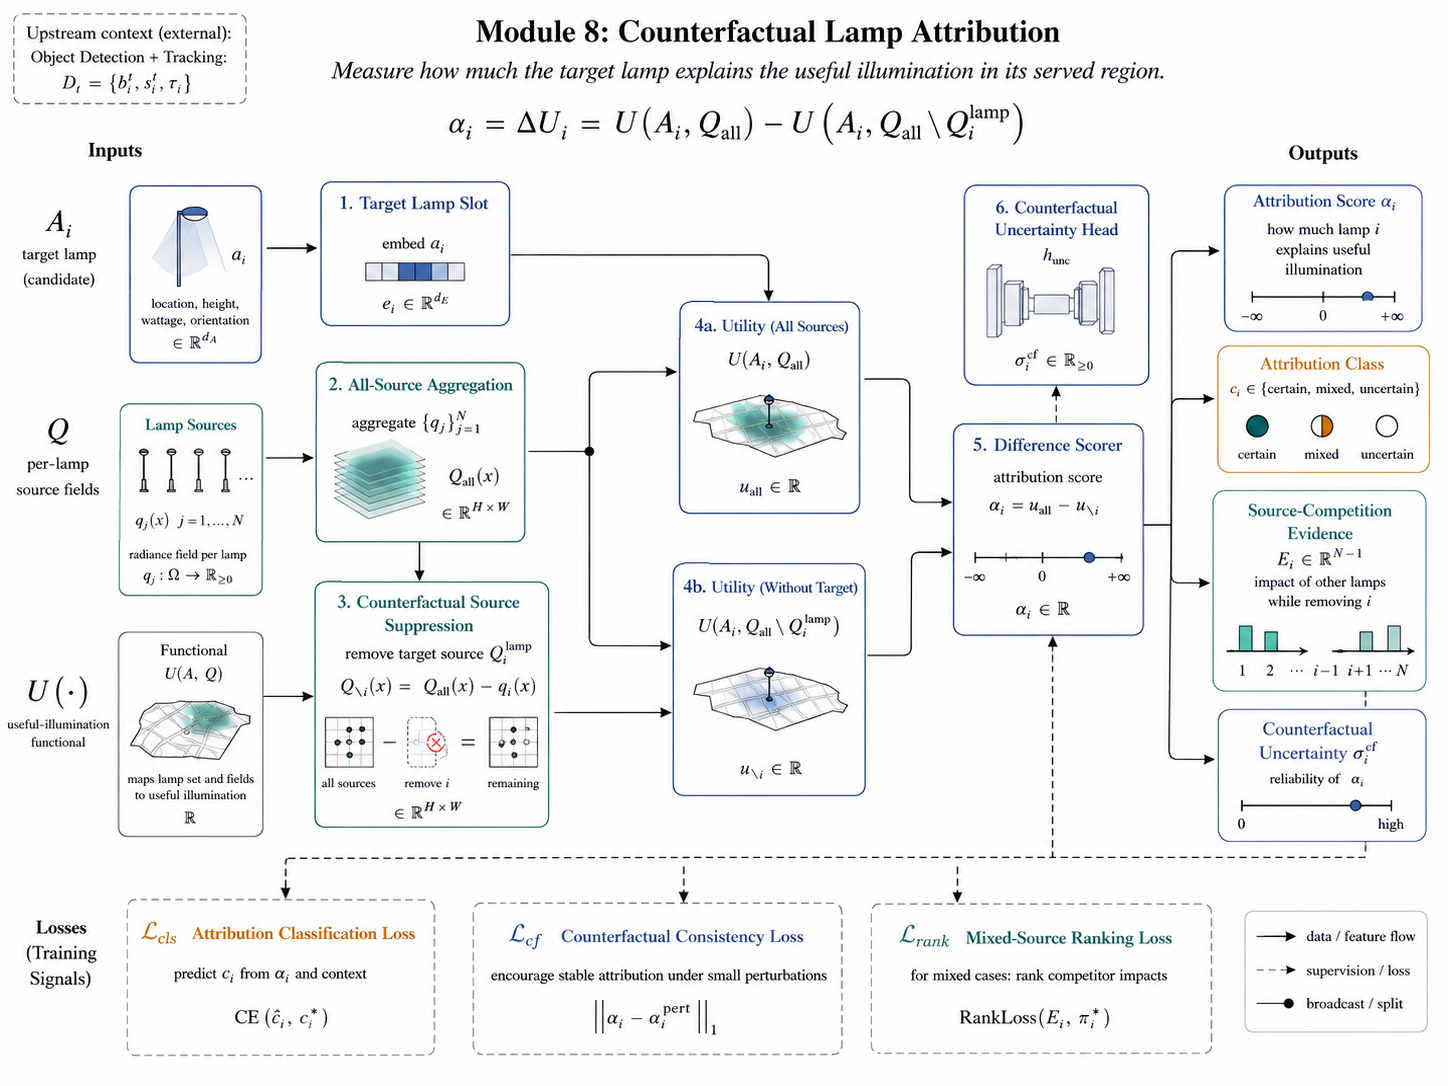
\includegraphics[width=\textwidth]{figures/module_8.png}
\captionof{figure}{Counterfactual lamp attribution. The module compares useful illumination with all source fields against useful illumination after suppressing the target-lamp source field.}
\label{fig:module-counterfactual-attribution}
\end{center}

This figure is the strongest pointer for mixed-source scenes: if removing the target lamp does not materially change the served-region utility, the system should lower attribution confidence.

\subsection{Monotonic scene-graph fusion}

The final fusion model represents the scene as a graph:
\[
G_{\omega}(V,E,h_i,\alpha_i) \rightarrow (y_i,c_i,\Omega_i),
\]
where \(V\) contains lamp, road, footpath, crossing, confounder, camera, geometry, and route nodes; \(E\) contains typed edges such as \texttt{serves}, \texttt{overlaps}, \texttt{confounds}, \texttt{observed\_by}, and \texttt{adjacent\_to}; \(y_i\) is the useful-illumination class; \(c_i\) is confidence; and \(\Omega_i\) is the uncertainty set.

The fusion head enforces monotonic constraints:
\begin{align*}
\frac{\partial score}{\partial coverage} &\geq 0, \\
\frac{\partial score}{\partial uniformity} &\geq 0, \\
\frac{\partial score}{\partial attribution} &\geq 0, \\
\frac{\partial score}{\partial glare} &\leq 0, \\
\frac{\partial score}{\partial confounder} &\leq 0, \\
\frac{\partial confidence}{\partial uncertainty} &\leq 0.
\end{align*}
This retains interpretability and prevents an unconstrained black-box model from learning unsafe relationships.

Figure~\ref{fig:module-scene-graph-fusion} presents the graph fusion layer and its monotonic constraints over coverage, uniformity, attribution, glare, confounders, and uncertainty.

\begin{center}
\centering
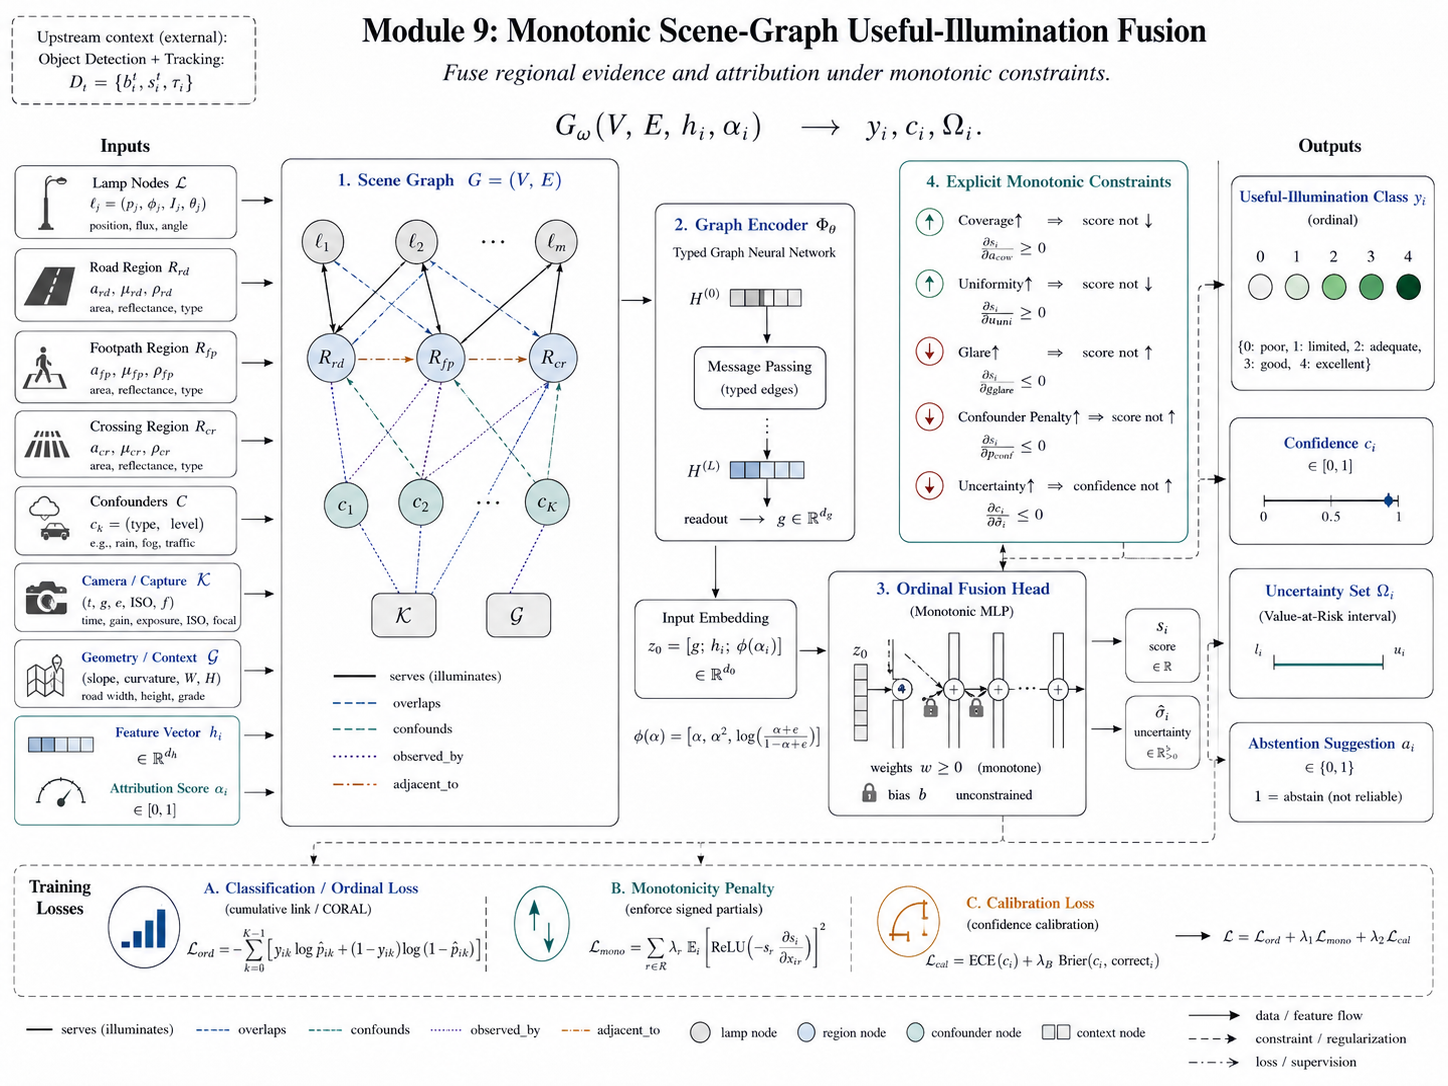
\includegraphics[width=\textwidth]{figures/module_9.png}
\captionof{figure}{Monotonic scene-graph useful-illumination fusion. Typed graph nodes and edges combine lamp, public-space, confounder, camera, geometry, and route evidence under explicit monotonic constraints.}
\label{fig:module-scene-graph-fusion}
\end{center}

The diagram ties component scores to the final ordinal class and confidence while preserving the policy that more glare, more confounding, or more uncertainty cannot improve the reported reliability.

\subsection{Group-conditioned conformal calibration and abstention}

The uncertainty layer maps model outputs into calibrated prediction sets:
\[
\Upsilon(y_i,c_i,d,r,mode) \rightarrow (\Omega_i,a_i),
\]
where \(d\) is device, \(r\) is route group, \(mode\) is capture mode, \(\Omega_i\) is a conformal prediction set, and \(a_i\in\{report,abstain\}\).

Calibration groups include phone model, capture mode, route, weather/wetness, confounder density, GPS quality, HDR/night-mode state, and road class. The layer supports selective risk curves: as the system abstains more, error should drop. This is essential for municipal use because high-confidence reports must be demonstrably more reliable than low-confidence reports.

Figure~\ref{fig:module-uncertainty-abstention} shows the grouped calibration, conformal prediction-set, abstention, and physical-validity gates behind this uncertainty layer.

\begin{center}
\centering
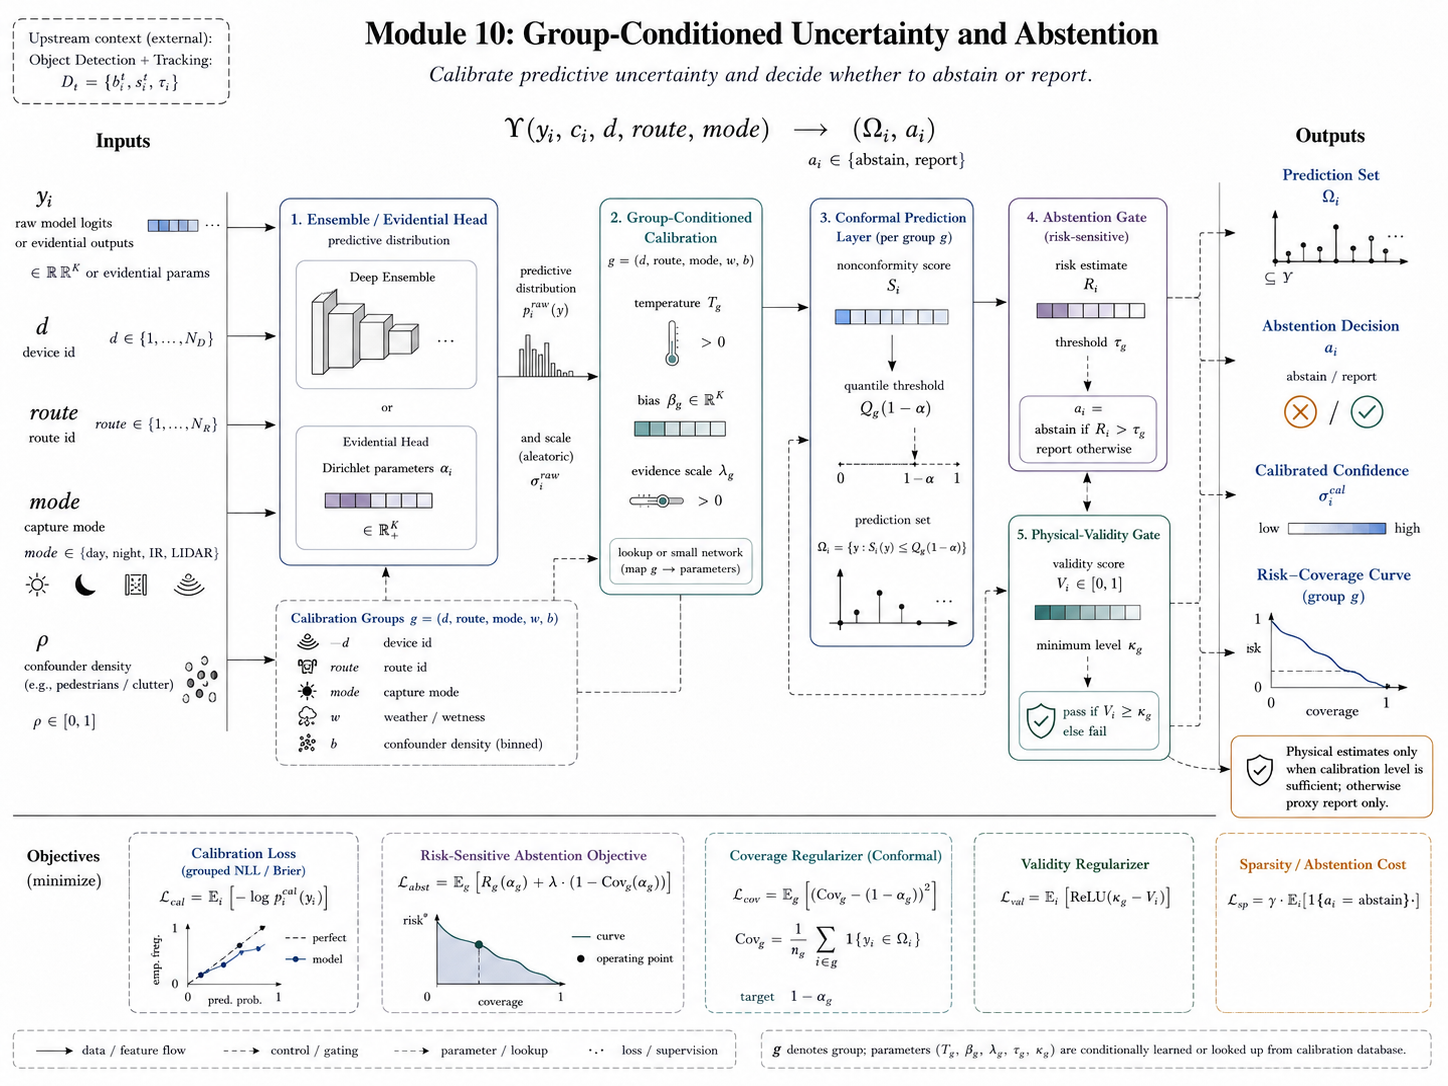
\includegraphics[width=\textwidth]{figures/module_10.png}
\captionof{figure}{Group-conditioned uncertainty and abstention. The module calibrates confidence by device, route, capture mode, weather, and confounder density, then decides whether to report or abstain.}
\label{fig:module-uncertainty-abstention}
\end{center}

This figure should guide implementation of selective reporting: proxy reports may be emitted at lower calibration levels, while physical estimates must pass the separate validity gate.

\subsection{Optional sparse-reference neural photometric field}

Physical estimates are optional and active only under calibrated capture. The model predicts:
\[
\Phi_{\zeta}(x\given A_i,Q,Z,C) \rightarrow \widehat{E}_i(x), \Sigma_E(x),
\]
where \(x\) is a ground-plane coordinate, \(Z=\{(x_j,E_j)\}\) are sparse lux-meter references, \(\widehat{E}_i(x)\) is approximate illuminance, and \(\Sigma_E(x)\) is uncertainty.

Constraints include non-negativity, spatial smoothness, weak distance decay, occlusion-aware attenuation, source additivity, and uncertainty increasing away from reference points. The output is invalid unless calibration level, metadata quality, geometry, and reference data satisfy the policy gate.

Figure~\ref{fig:module-calibration-bridge} places the optional physical-estimate path behind a calibration and physical-scale bridge.

\begin{center}
\centering
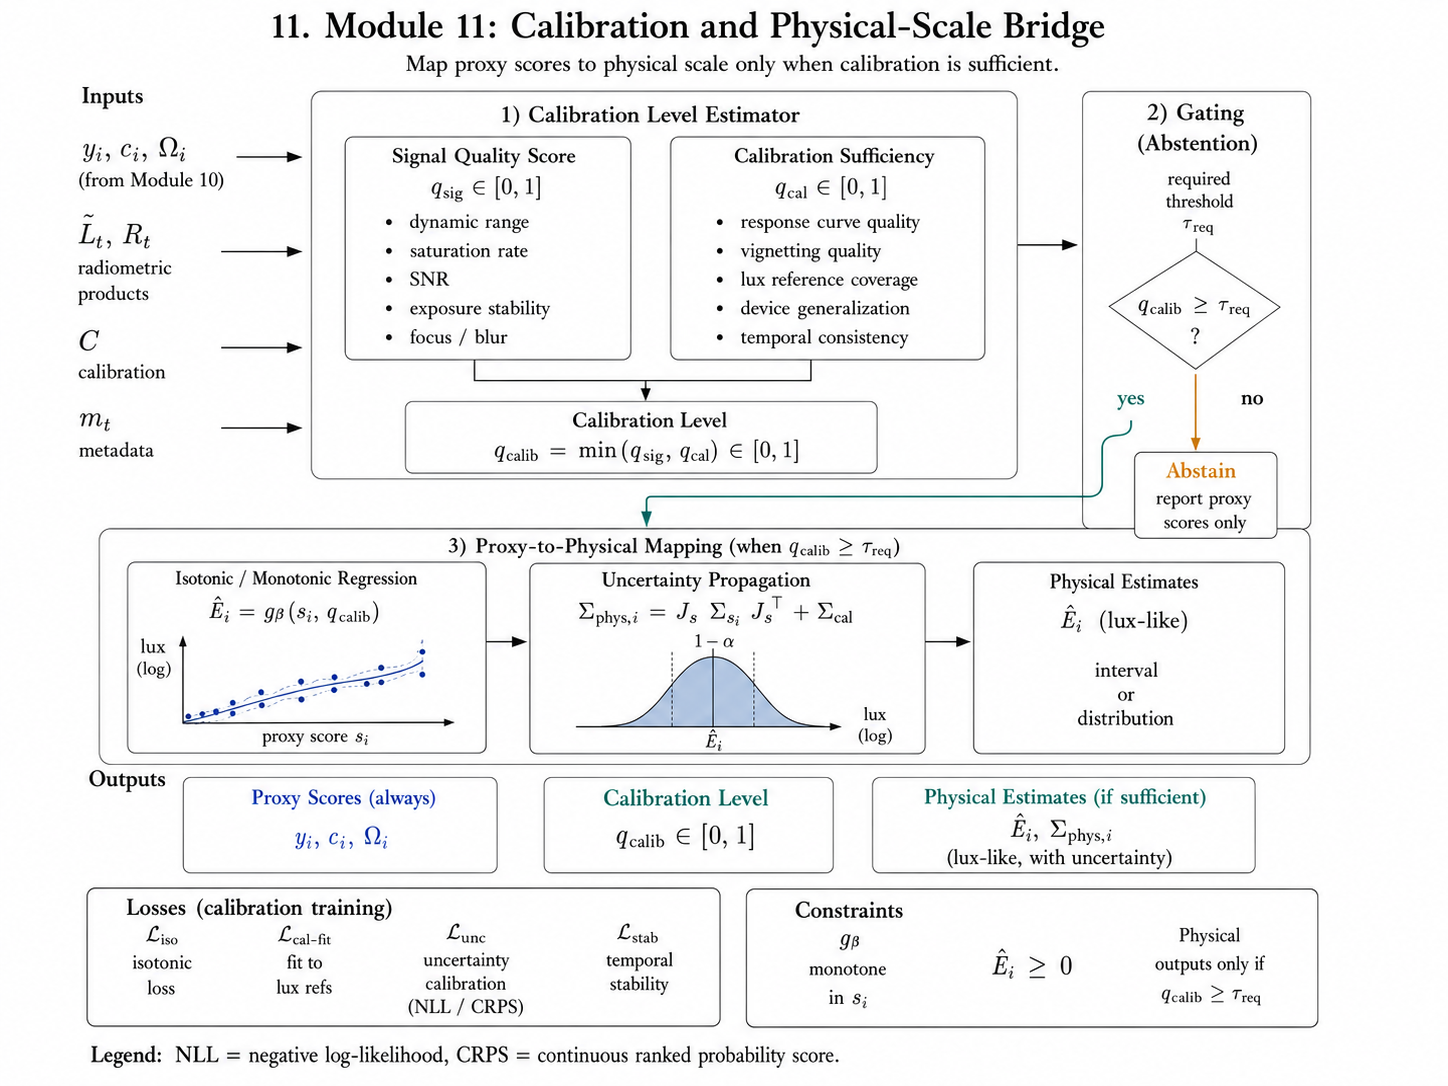
\includegraphics[width=\textwidth]{figures/module_11.png}
\captionof{figure}{Calibration and physical-scale bridge. Proxy scores are always available, but proxy-to-physical mapping and lux-like estimates are emitted only when signal quality and calibration sufficiency pass the required threshold.}
\label{fig:module-calibration-bridge}
\end{center}

This bridge reinforces the document's claim policy: calibrated physical outputs are a gated extension of the measurement block, not the default interpretation of ordinary phone video.

\subsection{Route-level graph aggregation}

Repeated passes are aggregated by:
\[
R_{\rho}(\{\R_i^{pass}\}) \rightarrow \overline{\R}_{\ell},
\]
where \(\overline{\R}_{\ell}\) is the refined route-level or physical-lamp report. The graph contains lamp-track observations, candidate physical pole nodes, road-segment nodes, drive-pass nodes, GPS neighborhoods, and map-prior nodes. This improves stability, duplicate merging, and manual-review prioritization.

\section{Model choices: stronger research model and long-term version}

\subsection{Stronger research model}

The stronger research model should use the full modular architecture but remain trainable with a realistic dataset. It should include:
\begin{itemize}
  \item metadata-conditioned radiometric normalization with device adapters and monotonic response inverse;
  \item latent emission-state temporal model over lamp crops;
  \item illumination-disentangled segmentation with raw and auxiliary enhanced branches;
  \item lamp-conditioned footprint field using cross-attention from lamp tokens to public-space tokens;
  \item neural source/confounder decomposition with temporal source slots;
  \item distributional coverage and uniformity estimator with quantile heads;
  \item counterfactual attribution head using source suppression;
  \item monotonic scene-graph fusion;
  \item group-conditioned conformal calibration and abstention.
\end{itemize}

The model should not be a monolithic end-to-end clip classifier. The component structure is necessary for scientific traceability, field debugging, and policy validity. The most important research claim is that explicit footprint, source decomposition, and counterfactual attribution improve per-lamp useful-illumination estimates in mixed-light nighttime scenes.

\subsection{Long-term version}

The long-term version adds stronger geometry, physical references, and municipal-scale aggregation:
\begin{itemize}
  \item custom Android Camera2 capture with locked exposure, YUV/RAW support, metadata logging, GPS/IMU sync, and calibration profile support;
  \item visual-inertial odometry or local SLAM for better camera trajectory and ground-plane reconstruction;
  \item pole inventory and road-segment GIS integration;
  \item sparse-reference neural photometric fields for calibrated sites;
  \item source-level temporal consistency across multiple passes;
  \item route-level graph aggregation over repeated observations;
  \item standards-aware screening reports with uncertainty, not automatic compliance certification.
\end{itemize}

The long-term system can emit approximate physical estimates only in calibrated mode. In all other modes, it remains a useful-illumination triage and auditing system.

\section{Dataset and annotation protocol}

\subsection{What must be collected}

The dataset must be built around useful illumination and attribution, not only lamp detection. The required data layers are:
\begin{itemize}
  \item nighttime video from multiple phone models and capture modes;
  \item synchronized camera metadata, GPS, IMU, and detector tracks;
  \item repeated passes over the same routes on different nights;
  \item varied road classes: residential, arterial, market, campus, footpath-heavy, crossing-heavy, tree-lined, underpass, and mixed commercial corridors;
  \item varied lighting layouts: one-sided, staggered, median, high-mast, dense adjacent lamps, decorative lighting;
  \item varied conditions: dry, wet, low traffic, high traffic, headlights, shopfronts, vegetation occlusion, parked vehicles, reflective surfaces;
  \item optional municipal data: pole locations, lamp type, height, arm length, wattage, road class, outage logs, maintenance history;
  \item calibrated reference subsets with lux-meter measurements and controlled capture;
  \item annotations for public-space semantics, source/confounders, occlusion, affected regions, task visibility, and attribution confidence.
\end{itemize}

The dataset should be layered: scalable capture first, calibrated reference sites second, dense annotation third, municipal linkage fourth. This is an adoption from the report analysis and should be kept because it makes the project feasible without sacrificing scientific validation.

\subsection{Lux-meter reference protocol}

The lux-meter reference protocol has stationary and mobile components.

\textbf{Stationary reference.} This is the decisive protocol for per-lamp attribution. Select representative lamp sites and measure a grid of points across carriageway, footpath, crossing, verge, and between-lamp regions. Collect horizontal illuminance at ground level and vertical illuminance at approximately pedestrian face height where pedestrian visibility matters. Record site geometry, timestamp, weather, surface condition, traffic state, nearby confounders, lamp layout, and phone capture mode.

\textbf{Mobile reference.} A vehicle-mounted or walking lux meter can record corridor-level variation and help synchronize video with broad light exposure trends. It should not be treated as sufficient per-lamp ground truth because it cannot isolate individual lamp contributions in dense mixed-source environments.

Each calibrated site should include:
\begin{itemize}
  \item points under the lamp;
  \item midpoint between adjacent lamps;
  \item near-side and far-side footpath;
  \item crossing approach if present;
  \item darkest visible public-space patch;
  \item brightest non-saturated ground patch;
  \item points inside and outside the estimated served region;
  \item repeated readings to estimate instrument and operator variability.
\end{itemize}

Sparse lux points should be used for calibration, threshold learning, physical validation, and uncertainty checking. They should not be treated as dense pixel-level ground truth.

\subsection{Visibility and task labels}

Useful illumination is task-conditioned. The labels should include:
\begin{itemize}
  \item footpath adequate for safe walking;
  \item carriageway adequate for lane edge and obstacle visibility;
  \item crossing adequate for seeing a pedestrian or cyclist;
  \item obstacle visibility;
  \item pedestrian upper-body or face-height visibility proxy;
  \item route-boundary visibility;
  \item perceived dark-zone risk;
  \item discomfort-glare likelihood.
\end{itemize}

Labels should use ordinal scales and pairwise rankings. Pairwise rankings are valuable because annotators can often say that one lamp-region observation is better than another more reliably than they can assign an absolute class.

\subsection{Semantic and confounder labels}

Semantic labels should include road, footpath, crossing, curb, verge, median, vegetation, vehicle, parked vehicle, building, shopfront, window, sign, billboard, traffic signal, sky, wet/reflection-like road, occluder, and unknown.

Confounder labels should include headlight, taillight, shopfront, window, signage, traffic signal, billboard, decorative light, wet-road reflection, other streetlight, and unknown bright source. Labels should support both masks and boxes. Temporal labels should mark moving headlights, transient flares, and persistent static confounders.

\subsection{Attribution confidence labels}

Attribution labels should be attached to affected-region annotations, not merely whole frames. Suggested classes are:
\begin{itemize}
  \item certain target-lamp attribution;
  \item likely target-lamp attribution;
  \item mixed attribution;
  \item likely non-target source;
  \item uncertain/invalid.
\end{itemize}

Annotators should not be forced to assign a single lamp when the scene is genuinely mixed. The model must learn uncertainty rather than inventing certainty.

\section{Evaluation protocol}

\subsection{Physical metrics}

Physical metrics are computed only on calibrated subsets. They include:
\begin{itemize}
  \item mean absolute error and RMSE for horizontal illuminance;
  \item mean absolute error and RMSE for vertical illuminance where available;
  \item rank correlation for relative illuminance ordering;
  \item threshold agreement for underlit versus acceptable regions;
  \item uncertainty interval coverage;
  \item calibration curves for optional physical estimates.
\end{itemize}

Results must be stratified by device, capture mode, road type, wet/dry condition, confounder density, calibration level, and route.

\subsection{Task-usefulness metrics}

Task-usefulness metrics include macro F1, balanced accuracy, weighted kappa for ordinal labels, AUROC/AUPRC for poor or dark detection, and rank correlation with human/task labels. Separate metrics should be reported for road, footpath, crossing, and mixed public-space tasks. The most important operational error is falsely labeling poor illumination as adequate.

\subsection{Attribution metrics}

Attribution metrics include affected-region mask IoU, boundary F-score, winning-lamp accuracy in overlapping-lamp scenes, false attribution under headlights/shopfronts, source-confusion error rate, attribution-class F1, and performance stratified by number of nearby lamps and confounder density.

The system should have a dedicated hard subset containing dense commercial lighting, moving headlights, adjacent lamps, tree occlusions, wet roads, and severe saturation.

\subsection{Temporal stability}

Temporal metrics include track-level score variance, category flip rate, status duty-cycle accuracy, flicker detection F1, repeat-drive consistency, score jitter after exposure normalization, and track-fragmentation sensitivity. A stable lamp should not produce unstable reports unless the evidence itself is unstable.

\subsection{Calibration and uncertainty}

Calibration metrics include expected calibration error, Brier score where appropriate, selective risk under abstention, risk-coverage curves, conformal prediction-set coverage, group-conditioned coverage, and out-of-distribution detection rate. Calibration must be evaluated by device, route, capture mode, road class, wetness, HDR/night-mode state, and confounder density.

\subsection{On-device latency, memory, and energy}

Deployment metrics include end-to-end latency, module-wise latency, p50/p95 latency, RAM usage, model size, energy per minute, sustained thermal behavior, battery drain, and FPS under realistic detector-plus-measurement scheduling. Measurements should be taken on representative Android devices and under sustained capture, not only short synthetic runs.

\section{Baselines that the system must beat}

The system must beat simple baselines, especially in hard mixed-source scenes.

\begin{center}
\scriptsize
\begin{tabular}{p{0.27\textwidth}p{0.31\textwidth}p{0.31\textwidth}}
\toprule
\textbf{Baseline} & \textbf{What it tests} & \textbf{Why the full system should beat it} \\
\midrule
Detector status only & Predict usefulness from on/off/dim/flicker status. & Ignores served region, uniformity, confounders, and task adequacy. \\
Raw lamp-box brightness & Use source crop brightness as utility. & Confused by exposure, saturation, bloom, and camera response. \\
Exposure-normalized lamp-box brightness & Metadata-aware source brightness shortcut. & Still ignores ground region, attribution, and confounders. \\
Scene-average road brightness & Estimate route light from road-mask brightness. & Cannot assign useful illumination to a specific lamp. \\
Segmentation-only brightness & Use road/footpath brightness without lamp footprint. & Fails where nearby lamps or shops illuminate the region. \\
Naive geometric cone/ellipse & Project a fixed served region from lamp position. & Fails under occlusion, weak geometry, road layout changes, and mixed sources. \\
No-confounder model & Full model without source/confounder decomposition. & Tests whether explicit confounder reasoning improves hard cases. \\
No-counterfactual model & Full model without counterfactual attribution. & Tests whether source suppression improves attribution confidence. \\
Ambient-light sensor route proxy & Use phone ALS or broad route-level light measurement. & Useful at corridor level, not per-lamp attribution. \\
Direct physical regression & Regress lux from brightness features on calibrated subset. & Tests whether structured photometric fields and uncertainty beat naive regression. \\
\bottomrule
\end{tabular}
\end{center}

The proposed architecture must show improvement on average and especially on confounder-heavy, adjacent-lamp, wet-road, occluded, and exposure-unstable subsets.

\section{Failure modes and mitigations}

\begin{center}
\scriptsize
\begin{tabular}{p{0.26\textwidth}p{0.61\textwidth}}
\toprule
\textbf{Failure mode} & \textbf{Mitigation} \\
\midrule
Auto-exposure, HDR, and night-mode distort brightness. & Use metadata-conditioned normalization, exposure-jump flags, reliability masks, calibration tiers, and abstention from physical estimates. \\
Saturation and bloom hide source intensity. & Treat saturation as uncertainty and glare evidence, not brightness evidence; predict intervals for clipped pixels. \\
Enhancement changes measurement features. & Use enhancement only as auxiliary segmentation/confounder input; sample measurement features from original or normalized capture. \\
Headlights and moving vehicles contaminate road brightness. & Use temporal source decomposition, vehicle/headlight masks, motion cues, and counterfactual attribution. \\
Shopfronts, signs, and windows dominate sidewalk light. & Use semantic confounder masks and source slots; penalize static non-lamp contribution in served regions. \\
Wet roads and reflections create false bright regions. & Add wet/reflection labels, source-reflection slots, reflection geometry cues, and uncertainty flags. \\
Adjacent lamps overlap. & Use lamp-conditioned footprint fields, source decomposition, graph edges between lamps and regions, and mixed-attribution classes. \\
Vegetation or buildings occlude lamp or footprint. & Use occluder masks, occlusion gates in \(A_i(p)\), crop occlusion probabilities, and footprint-quality downgrading. \\
Poor segmentation breaks region estimates. & Use segmentation uncertainty, abstention, and no high-confidence reporting when public-space masks are invalid. \\
Weak geometry breaks ground projection. & Emit image-space regions when ground-plane quality is low; suppress ground polygons and physical estimates. \\
Detector misses lamps. & Never infer off status from missing detections; carry observation-completeness flags. \\
Track fragmentation creates duplicate reports. & Merge fragments at pass-level using temporal, spatial, visual, and GPS continuity. \\
Phone/device variation shifts brightness. & Use device adapters, device-held-out evaluation, calibration profiles, and group-conditioned calibration. \\
GPS drift corrupts map assignment. & Preserve GPS uncertainty; aggregate by route segment; avoid precise pole IDs without map support. \\
Task mismatch hides pedestrian risk. & Report road, footpath, crossing, and public-space adequacy separately. \\
\bottomrule
\end{tabular}
\end{center}

\section{Deployment plan}

\subsection{Desktop research implementation}

The desktop implementation should be a Python package independent of detector internals. It consumes detector outputs through a stable adapter and writes reports, overlays, masks, features, and metrics.

Recommended structure:

\begin{lstlisting}
src/rbccps_measurement/
  contracts/
    input_schema.py
    output_schema.py
    calibration_policy.py
  ingest/
    video_reader.py
    frame_store.py
    detector_interface.py
    sync.py
    validation.py
  normalization/
    luma.py
    exposure.py
    radiometric_inverse.py
    saturation_bloom.py
  status/
    crop_buffer.py
    latent_emission_state.py
  segmentation/
    illumination_disentangled_segmenter.py
    masks.py
  geometry/
    pose.py
    ground_plane.py
    lamp_footprint_field.py
  decomposition/
    source_slots.py
    task_supervised_decomposition.py
  features/
    distributional_coverage.py
    adequacy.py
    uniformity.py
    glare.py
    occlusion.py
    temporal.py
  attribution/
    counterfactual.py
  fusion/
    scene_graph.py
    monotonic_heads.py
    conformal.py
    abstention.py
  photometry/
    sparse_reference_field.py
  route/
    graph_aggregation.py
  reporting/
    json_writer.py
    csv_writer.py
    geojson_writer.py
    overlays.py
  evaluation/
    physical_metrics.py
    task_metrics.py
    attribution_metrics.py
    temporal_metrics.py
    calibration_metrics.py
    baselines.py
  cli/
    measure_clip.py
    measure_batch.py
    evaluate.py
\end{lstlisting}

Example commands:

\begin{lstlisting}
python -m rbccps_measurement.cli.measure_clip \
  --video data/videos/drive_001.mp4 \
  --detections runs/detector/drive_001_tracks.json \
  --metadata data/metadata/drive_001_camera.json \
  --imu data/metadata/drive_001_imu.csv \
  --gps data/metadata/drive_001_gps.csv \
  --calibration configs/device_calibration.yaml \
  --out runs/measurement/drive_001
\end{lstlisting}

\begin{lstlisting}
python -m rbccps_measurement.cli.evaluate \
  --pred runs/measurement/drive_001/reports.json \
  --gt data/annotations/drive_001_measurement_gt.json \
  --out runs/measurement_eval/drive_001
\end{lstlisting}

\subsection{Android/TFLite or edge deployment}

The edge version should use a custom Camera2-style capture path wherever possible. It should log YUV frames or RAW where supported, exposure metadata, ISO, focal length, AE/AWB/HDR state, GPS, IMU, and calibration profile ID. If only arbitrary gallery video is available, the system must fall back to Tier 0 behavior.

On-device inference should use quantized segmentation, status, source/confounder, and fusion models. The scheduler should run detector/tracker every frame or at the existing upstream cadence, status on short windows, segmentation every few frames, geometry when pose changes, and fusion when enough track evidence is available. Reports can be emitted on-device, with raw video upload disabled by default unless explicit research consent exists.

\subsection{Offline batch mode}

Offline batch mode is a first-class deployment path. It is the safest way to validate the measurement block before mobile integration. It accepts detector JSON, original video, metadata logs, and optional calibration; processes clips corridor by corridor; and emits JSON, CSV, GeoJSON, overlays, and feature snapshots. Batch mode can use stronger models than on-device mode and should be the default for research evaluation.

\subsection{Integration with object-detection block outputs}

The measurement block integrates through a thin contract. It does not import detector internals. It requires original-frame coordinates, frame IDs, timestamps, bbox format, detector score, track ID, track confidence, track age, lost count, source model, and optional detector cue scores. It should explicitly validate coordinate systems and reject inconsistent manifests. If the upstream detector uses enhanced views internally, it must map detections back to original-frame coordinates before measurement.

\section{Open questions and assumptions}

The main assumptions are:
\begin{itemize}
  \item the detector can provide stable track IDs and original-frame bounding boxes;
  \item camera metadata can be logged for research captures;
  \item at least a subset of routes can be captured with controlled Camera2-style settings;
  \item calibrated reference measurements can be collected at selected sites;
  \item public-space task labels and attribution labels can be annotated with sufficient quality;
  \item municipal GIS, pole metadata, and outage logs may be unavailable initially and must remain optional.
\end{itemize}

The main open questions are:
\begin{enumerate}
  \item Which operational road and pedestrian-space classes should define adequacy thresholds?
  \item Will RBCCPS deploy a custom Android capture app, or must the first release support arbitrary videos only?
  \item How many calibrated sites are feasible for the first field campaign?
  \item Can pole inventory, lamp height, wattage, and road-class metadata be obtained from municipal sources?
  \item Should the first publication emphasize source attribution, calibrated proxy measurement, route-level auditing, or all three?
  \item What abstention rate is acceptable for a municipal pilot?
  \item What privacy policy governs raw video, faces, vehicle plates, and shopfronts?
\end{enumerate}

The recommended answer to the publication question is: emphasize source attribution and uncertainty-aware useful-illumination assessment as the core novelty; present calibrated physical estimation as an optional extension; and present mobile/route deployment as the operational validation path.

\section*{Final recommendation}
\addcontentsline{toc}{section}{Final recommendation}

The final architecture should combine the report's system discipline with the ML novelty modules developed in this design process. The report's strongest contributions are clip-centered contracts, calibration-tier claim policy, original-frame measurement discipline, observation-completeness flags, track-pass-inventory state, asymmetric scheduling, layered dataset design, and leakage-safe evaluation. The strongest novel ML contributions are lamp-conditioned footprint fields, neural source decomposition, counterfactual attribution, monotonic scene-graph fusion, metadata-conditioned radiometric inversion, illumination-disentangled segmentation, distributional coverage modeling, group-conditioned conformal calibration, sparse-reference photometric fields, and route-level graph aggregation.

The final research identity should be stated as follows: the RBCCPS measurement block is not a lux meter and not merely a detector add-on. It is an uncertainty-aware, per-lamp useful-illumination attribution system for mixed-source urban nighttime video.

\end{document}
